%! TeX program = lualatex
%---------------------------ALLGEMEINE IMPORTS-------------------------------------
\documentclass[12pt,english,ngerman]{scrartcl}

\usepackage{iftex}

% text input and font
\ifluatex  % LuaLaTeX
    \usepackage{fontspec}
    % main font automatically: Latin Modern
    %\setmonofont{Consolas}
    % \newfontfamily{\Consolas}{Consolas}
\else  % pdfLaTeX
    \usepackage[utf8]{inputenc}  % input in UTF-8
    \usepackage[T1]{fontenc}  % output in T1 fonts (west European encoding)
    \usepackage{lmodern}  % Latin modern font for main text
    \usepackage[mono]{zi4}  % Consolas font for monospaced text
    % \newfontfamily{\Consolas}{\fontfamily{zi4}}
\fi

% text processing
\usepackage{babel}  % language package
\usepackage[intlimits]{mathtools}  % upgrade of amsmath (automatically loaded) - \int^_ like \limits^_
\usepackage{amssymb}  % upgrade of amsfonts (American Math Society)
\usepackage{amstext}  % \text command in math environments
%\usepackage{bm}  % bold math fonts
% \LetLtxMacro{\svqty}{\qty}
% \usepackage{physics}  % macros for easier typesetting of physical formulas
% \LetLtxMacro{\qty}{\svqty}
\usepackage{letltxmacro}  % \let command for robust macros (new sqrt)
\usepackage{chemformula}  % typeset chemical formulas
\usepackage{microtype}


% page geometry
\usepackage{scrlayer-scrpage}  % page formatting with KOMA options
\usepackage[paper=a4paper, hmargin=3cm, vmargin=2.5cm, includehead, includefoot, head=29pt]{geometry}  % horizontal: 3cm, vertical: 2.5cm strict with or without headers and footers
\usepackage{tabto}  % tab stops
\NumTabs{8}  % 8 equally spaced of \textwidth tab stops



% floats
\usepackage[hypcap=false, labelfont=bf]{caption, subcaption}  % caption editing - hypcap warning with hyperref
\usepackage{float}  % for [H] (forced here) specifier
\usepackage{tabularray}
\usepackage{diagbox}  % table cells with diagonal lines


% graphical input
\usepackage{graphicx}  % input JPEG, PNG, PDF, etc.
\usepackage{pdfpages}  % input PDF as whole pages
\usepackage{lastpage}  % reference to last page
\usepackage{pgfplots}  % for tikzplotlib
\usepgfplotslibrary{groupplots,dateplot}
\usetikzlibrary{patterns,shapes.arrows}
\pgfplotsset{compat=newest}
\usepackage{import}


% text
\usepackage[locale=DE, uncertainty-mode=separate]{siunitx}  % SI units, German formatting - \pm stays \pm instead of ..(.)
\let\svqty\qty %dont import physics before siunitx is loaded
\usepackage{physics}
\let\qty\svqty
\usepackage{icomma}  % no space after commas instead of English points) in decimal values
\usepackage{enumitem}  % better enumerating with style options
\usepackage{nicefrac}  % inline-fractions in n/d-style
\usepackage{xcolor}  % custom colors
\usepackage{listings, scrhack}  % code display; listings in combination with KOMA
\usepackage{fancyvrb}  % Verbatim environment with better options (capital V!)

\usepackage{listings}

% literacy
\usepackage[bibencoding=auto,backend=biber,autolang=other]{biblatex}  % backend=Biber is standard
\usepackage{csquotes}  % better quotation - should also be used in combination with package babel (warning)
\usepackage{xurl}  % breaks links - after BibLaTeX, but before hyperref!
\usepackage[hidelinks]{hyperref}  % produces most errors, last to load
\usepackage{bookmark}


% KOMA setups
% header and footer
\pagestyle{scrheadings}  % KOMA style
\clearpairofpagestyles  % reset
\setkomafont{pageheadfoot}{\normalfont}  % standard font in header and footer
\setlength{\headheight}{29pt}  % just look at the warning
\cfoot{\pagemark{} / \pageref*{LastPage}}  % center foot - *: ref but no hyperlink
% {}: empty statement
% \ : protected space
% \,: small space
\DeclareTOCStyleEntry{dottedtocline}{section}  % sections in TableOfContents with dotted lines
\KOMAoptions{parskip=half-}  % paragraphs with half a line height space instead of indentation, last line with no special treatment


% package setups

% biblatex
%\addbibresource{files/JabRef_Database/physics.bib}
% \addbibresource{transistor.bib}

% rewrite names (babel overwrites German with standard English names, therefore at document beginn [after everything is loaded])
\AtBeginDocument{\renewcommand{\refname}{Literaturverzeichnis}}
% others:
% \contentsname
% \listtablename
% \listfigurename


% xcolor
\definecolor{code_keyword}{HTML}{A06E9D}
\definecolor{code_string}{HTML}{AD6E3E}
\definecolor{code_comment}{HTML}{6A9955}
%\definecolor{code_basic}{HTML}{D4D4D4}
%\definecolor{code_background}{HTML}{1E1E1E}

% siunitx
\DeclareSIUnit{\dig}{dig}  % digits for uncertainty of electronical measurement devices
\sisetup{locale = DE}  % deutschsprachige SI-Konvention
\sisetup{per-mode = fraction}
\DeclareSIUnit{\px}{px}
\DeclareSIUnit{\strich}{|||}

%Eigene Commands
\newcommand{\der}[2]{\frac{\mathrm{d}#1}{\mathrm{d}#2}}
\newcommand{\pder}[2]{\frac{\partial #1}{\partial #2}}

% listings
\lstdefinestyle{python}{
    %basicstyle=\Consolas\footnotesize,%\color{code_basic},  % \footnotesize contains \selectfont implicitly
    %backgroundcolor=\color{code_background},
    commentstyle=\color{code_comment},
    keywordstyle=\bfseries\color{code_keyword},
    numberstyle=\tiny,
    stringstyle=\color{code_string},
    breakatwhitespace=false,
    breaklines=true,
    captionpos=b,
    keepspaces=true,
    numbers=left,
    numbersep=5pt,
    showspaces=false,
    showstringspaces=false,
    showtabs=false,
    tabsize=2,
}
\lstset{style=python}
\ifPDFTeX
    \renewcommand*{\ttdefault}{lmvtt}  % Latin Modern Typewriter Proportional
\fi


% new sqrt
% https://en.wikibooks.org/wiki/LaTeX/Mathematics
\makeatletter
\let\oldr@@t\r@@t
\def\r@@t#1#2{%
    \setbox0=\hbox{$\oldr@@t#1{#2\,}$}\dimen0=\ht0
    \advance\dimen0-0.2\ht0
    \setbox2=\hbox{\vrule height\ht0 depth -\dimen0}%
    {\box0\lower0.4pt\box2}}
\LetLtxMacro{\oldsqrt}{\sqrt}
\renewcommand*{\sqrt}[2][\ ]{\oldsqrt[#1]{#2} }
\makeatother


% own commands
% \newcommand* can't contain multiple lines
% \newcommand can
\newcommand*{\mup}[1]{\ensuremath{\text{\textup{#1}}}}  % upright normal font in math mode
\newcommand*{\inkgraphics}[3][\linewidth]{\def\svgwidth{#1}\import{#2}{#3}}


% tabularray
% imports_and_setups{
%     expl3,
%     xparse,
%     ninecolors
%     \hypersetup{pdfborder={0 0 0}}
% }

% tabularray environments
\RequirePackage{tabularray}  % like \usepackage but for packages
\UseTblrLibrary{siunitx}  % siunitx suited for tabularray
\UseTblrLibrary{bookmark}  % bookmark suited for tabularray
% TRIPLE BRACKETS {{{}}} to protect strings from \num{} interpretation in S columns
\UseTblrLibrary{diagbox}  % diagbox suited for tabularray
\UseTblrLibrary{varwidth}  % measure cell width using package 'varwidth'

% standard environment
\SetTblrInner{
    hlines,
    vlines,
    columns={
            halign=c,
            valign=m,
        },
    measure=vbox,
}

% X columns
\NewTblrEnviron{tblrx}
\SetTblrInner[tblrx]{
    hlines,
    vlines,
    columns={
            halign=c,
            valign=m,
            co=1,  % coefficient of width for expendable columns (X columns)
        },
    width=\linewidth,
    vspan=minimal,
    measure=vbox,
}

% -X columns
\NewTblrEnviron{tblr-x}
\SetTblrInner[tblr-x]{
    hlines,
    vlines,
    columns={
            halign=c,
            valign=m,
            co=-1,  % shrinks X column down to natural width
        },
    width=\linewidth,
    vspan=minimal,
    measure=vbox,
}

% no hline and vline left and on top of first cell
\NewTblrEnviron{tblr_omit_first_cell}
\SetTblrInner[tblr_omit_first_cell]{
    hlines,
    vlines,
    columns={
            halign=c,
            valign=m,
        },
    hspan=even,
    vspan=minimal,
    %
    hline{1}={1}{white},  % first row, only first cell
    vline{1}={1}{white},
    measure=vbox,
}


\addbibresource{cmos.bib}
    % Kopfzeile
\ihead{SS22\\18.05.2022}
\chead{\textsc{Hinterleitner} Michael - 12002411 \\ \textsc{Philipp} Maximilian - 11839611}
\ohead{LU ECM-\\ CMOS Logik}
    % Fußzeile
%--------------------------------------AB HIER DOKUMENT---------------------------------------------
\begin{document}
% 
\includepdf{deckblatt3.pdf}
\tableofcontents
\newpage


%\section{Aufgabenstellung}\label{sec:Aufgabenstellung}

% Die nachfolgende Aufgabenstellung wurde von den Laborbetreuern bereitgestellt
% und beinhaltet sowohl Angaben zur Vorbereitung als auch zur praktischen
% Durchführung der Übung:

% zu 1: Aufgabenstellung Das vor der Übung verteilte Aufgabenblatt.
 
\includepdf[
     pages=-,  % all pages
     addtotoc={
         1, section, 1, Aufgabenstellung, sec:Aufgabenstellung
     }
 ]{angabe.pdf}

% zu 2: Vorbereitung Es sind beide Vorbereitungen dem Protokoll beizufügen.
% \section{Vorbereitung}\label{sec:Vorbereitung}
%Die folgende Vorbereitung wurde vor der Laborübung 
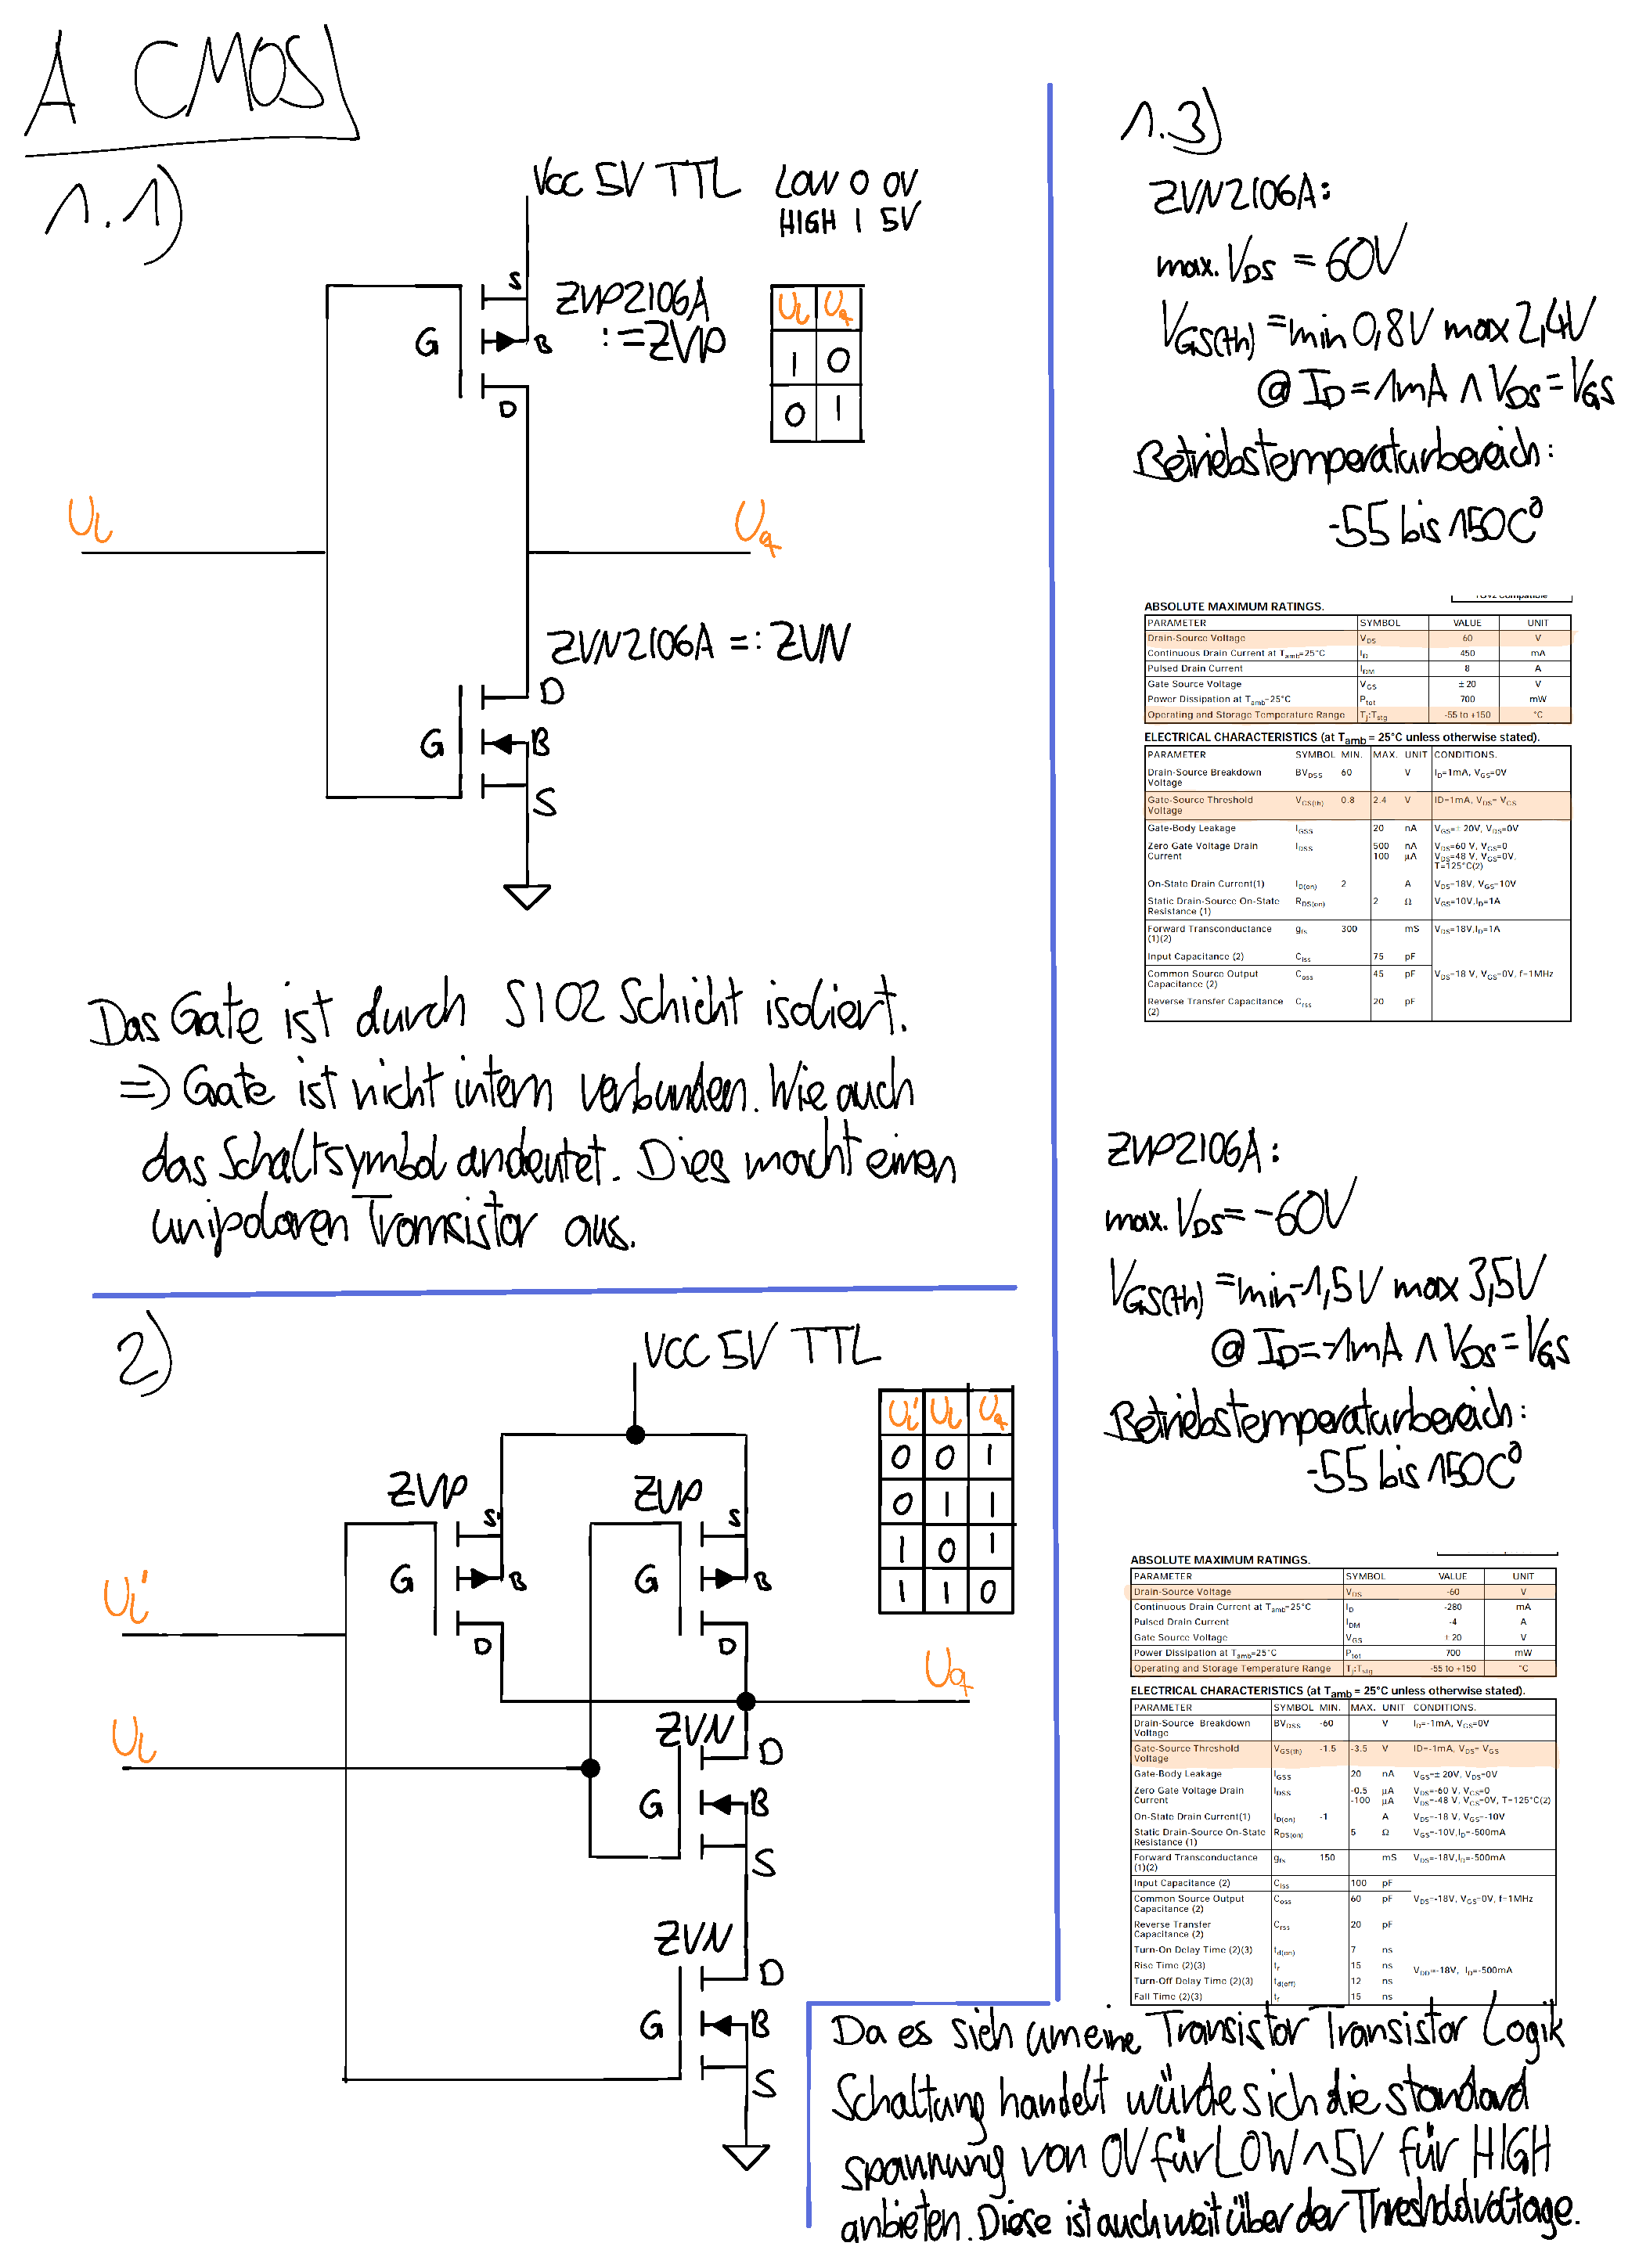
\includepdf[pages=-,
     addtotoc={
         1, section, 2, Vorbereitung, sec:Vorbereitung
     }]{./figures/CMOS-Logik1.pdf}
\includepdf[pages=-]{./figures/CMOS-Logik2.pdf}
% 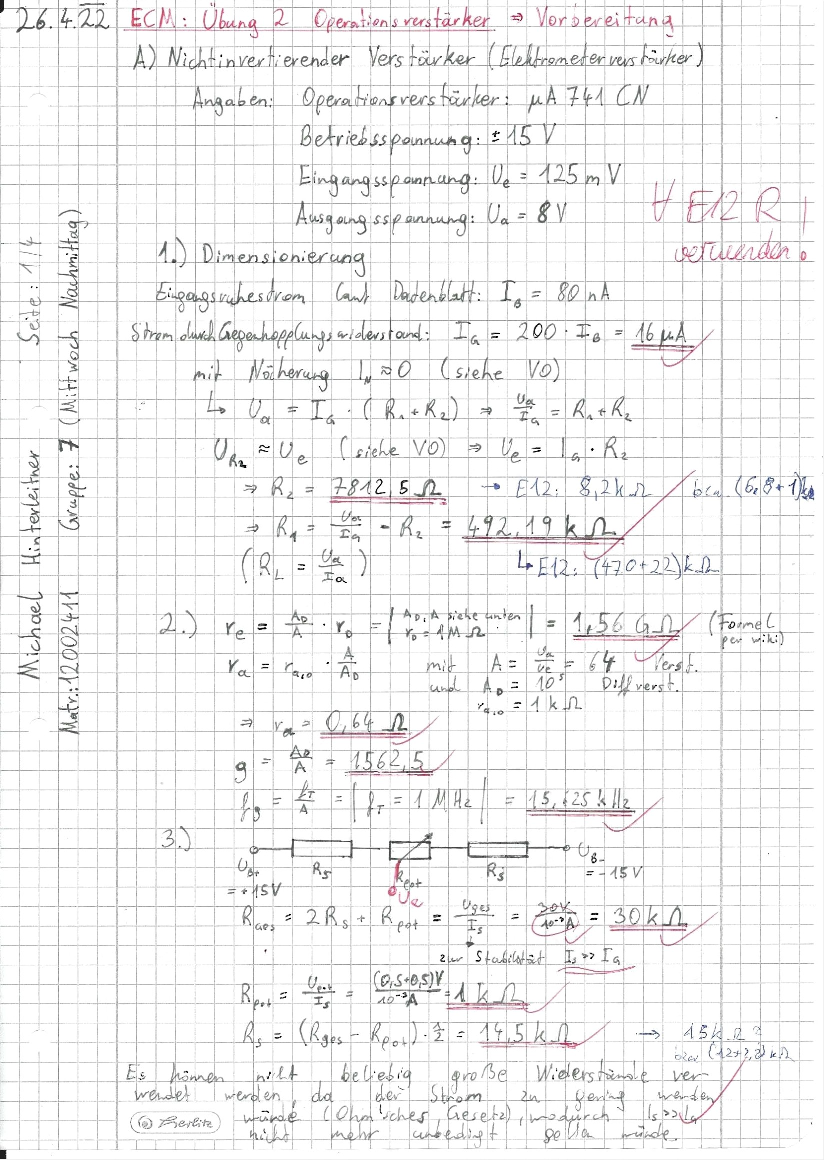
\includepdf[pages=-]{./mh_vorbereitung_opv.pdf}


% zu 3: Grundlagen In den Grundlagen sollen die später verwendeten Formeln
% stehen und kurz erklärt werden, dabei ist es nicht notwendig Formeln
% herzuleiten. Quellenangaben sind an dieser Stelle von Vorteil, weil Sie so
% schnell die betreffenden Stellen in Unterlagen finden. In den Rechnungen
% werden grundlegende Annahmen skizziert und begründet und dann mit diesen
% Annahmen, die für die Schaltungen notwendigen Werte berechnet. Dabei kann
% auch gleich auf die später wirklich verwendeten Werte Bezug genommen werden -
% wir verwenden bei den Widerständen zum Beispiel von den Normwert-Reihen die
% E12 und/oder E24 Serie (nach DIN 41426 bzw. IEC 63).
\section{Grundlagen}\label{sec:Grundlagen}
%%in Grundlagen
Operationsverstärker (kurz 'OPV oder 'OpAmp') dienen grundlegend der Verstärkung von 
Gleichspannungen. Sie besitzen einen nicht-invertierenden, der meist mit einem 
Plus, und einen invertierenden Eingang, der mit einem Minus dargestellt wird. Zu 
beachten ist, dass die Verstärkung auf die Differenzspannung der beiden Eingänge 
wirkt. Je zwei zusätzliche Anschlüsse finden sich für die positive und negative 
Betriebsspannung und für den Offsetabgleich, damit bei keiner Eingangsspannung 
auch keine Ausgangsspannung auftritt - dieser wird also in einer externen 
Schaltung durchgeführt.

\begin{figure}[H]
    \centering
    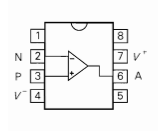
\includegraphics[width=6cm, height=6cm,keepaspectratio]{./figures/pics/pins.PNG}
    \caption{Schematische Darstellung der Pinbelegung eines klassischen Operationsverstärkers. Hierbei bezeichnet 2 den invertierenden, 3 den nicht-invertierenden Eingangskanal, 6 den Ausgang, 4 den Anschluss für die negative sowie 7 den Anschluss für die positive Betriebsspannung, 1 und 5 die Pins für den Offsetabgleich und 8 einen freien Pin.  \cite{tietze}}
    \label{fig:pin_anschl}
\end{figure}

In \autoref{fig:pin_anschl} sind die Pins eines Operationsverstärkers, wie er auch 
in der Laborübung verwendet wurde, zu sehen. Dabei ist zu beachten, dass jeder nicht 
belegte Pin auf Masse gelegt werden soll.

Es gibt vier grundlegende Arten der Verwendung von Operationsverstärkern, darunter
der nicht-invertierende Betrieb, bei dem das Eingangssignal nur auf den nicht-invertierenden 
Kanal gelegt wird und der invertierende auf Masse gelegt wird. Analog funktioniert der invertierende 
Modus, bei dem das Signal anstelle nun an den invertierenden Eingang gelegt wird, wodurch die Ausgangsspannung 
zusätzlich zur Verstärkung noch zum Eingangssignal invertiert wird. Beim Differenzbetrieb werden an 
beide Eingänge Signale angelegt und die Differenzspannung verstärkt. Im Falle des Gleichtaktbetriebs 
liegt das gleiche Eingangssignal an den beiden Eingängen an, wodurch es theoretisch keine Differenzspannung 
und Verstärkung geben sollte - in der Realität resultiert allerdings eine Verstärkung, die als 
Gleichtaktverstärkung bezeichnet wird.

Da der Operationsverstärker ohne zusätzliche Verkopplung sehr stark frequenzabhängig ist und 
nur eine geringe Bandbreite gewünscht verstärkt, wird eine Gegenkopplung vom Ausgang zum Eingang 
durchgeführt, wodurch die Verstärkung zwar abnimmt, die Bandbreite jedoch stark vergrößert wird. 
Die Bandbreite wird wie gewohnt durch die Grenzfrequenz charakterisiert, bei welcher die Verstärkung 
noch \SI{70}{\%} der maximalen beträgt. Wenn nun beispielsweise ein Kondensator in der Rückkopplung verbaut wird, 
handelt es sich um eine Integratorschaltung, die im zweiten Teil der Laborübung untersucht wird.

Die resultierende Verstärkung lässt sich gemäß \autoref{eq:ver} als Verhältnis der Ausgangs- $U_a$ zur Eingangsspannung $U_e$ berechnen.
\begin{equation}
	V=\frac{U_a}{U_e}
	\label{eq:ver}
\end{equation}

Die CMOS-Technologie basiert auf MOSFETs (Akronym für \textit{Metal Oxide
Semiconductor Field Effect Transistor}), also Feldeffekttransistoren (kurz FET)
mit einer Metalloxidschicht, die der Isolation der Halbleitermaterialien dient.
Analog zu den Bipolartransistoren, gibt es bei den Feldeffekttransistoren 3
Anschlüsse, nämlich Source, Gate und Drain. 
%Tietze Abbildung
FETs sind ebenso aus drei Halbleiterbereichen (p- respektive n-dotiert)
aufgebaut, die sich allerdings in ihrer Anordnung von den Bipolartransistoren
in der Hinsicht unterschieden, dass die Manipulationsrichtung normal zur
Stromflussrichtung liegt. Ein weiterer signifikante Unterschied zwischen den beiden
Typen von Transistoren ist, dass beim FET am Stromtransport nur noch eine Sorte
Ladungsträger, entweder Elektronen (n-MOSFET) oder Defektelektronen (p-MOSFET)
beteiligt sind. Weiters wird die Leitfähigkeit dieses Transistors über die
Gatespannung gesteuert - bei Bipolartransistoren erfolgt dies bekanntlich über
den Basisstrom. Zusätzlich wird zwischen Anreicherungs- und Verarmunsgtyp
unterschieden, welche gelegentlich auch als selbstleitend respektive
selbstsperrend bezeichnet werden. Dies beschreibt, wie die Bezeichnung
nahelegt, den Umstand, dass ein MOSFET ohne Manipulation über das Gate den
Strom entweder leitet oder sperrt. Aufgrund der Spannungssteuerung wird unter
anderem der Stromfluss reduziert, wodurch auch die Verlustleistung gering ist.
Dies ist auch ein großerer Vorteil der daraus aufgebauten CMOS-Technologie
(Akronym für \textit{Complementary Metal Oxide Semiconductor}), bei der stets
mindestents ein n- und p-MOSFET verwendet wird - so auch im ersten Teil dieser
Laborübung für den CMOS-Inverter und das NAND-Gatter. 

Bei Digitalschaltungen wird zwischen 2 Zuständen, \textit{High} und
\textit{Low} beziehungsweise 0 und 1, geschaltet. Mittels Logikgattern, die aus CMOS gebaut werden
können, können
Zustände beziehungweise weiterfolgend Eingangsvariablen verknüpft werden und in
der Folge Logiknetze konstruiert werden. Grundlegend für Schaltnetze sind die folgenden Gatter: AND, OR,
NOT, NAND und NOR, wobei auch ein Satz dieser genutzt werden kann, um ein anderes Gatter
zu erhalten; beispielsweise kann simpel aus einem AND und NOT ein NAND gebildet werden. Zur
Identifizierung und/oder Auswertung wird zu einer Logikschaltung eine
Wahrheitstabelle und eine Logikfunktion aufgestellt.

% zu 4: Versuchsdurchführung In diesem Punkt wird die Durchführung der
% einzelnen Aufgaben beschrieben. Im Simulationsteil ist die simulierte
% Schaltung mit allen Analyseparametern darzustellen. Im praktischen Teil sind
% die verwendete Geräte sowie die gemessenen Werte der verwendeten Bauteile
% anzugeben. Außerdem sind durchgeführte Funktionsüberprüfungen der Bauteile
% (Dioden, Transistor, etc.) anzuführen. Die Messergebnisse bzw. Oszillogramme
% sind mit Angabe der verwendeten Messgeräte anzugeben. Oszillogramme werden
% vom verwendeten Oszilloskop als Daten auf einen USB-Stick ausgegeben und
% können in das Protokoll aufgenommen werden. Das gleiche gilt für Schaltungen
% bzw. Ergebnissen von Simulationen. Es ist auf eine klare Darstellung der
% Messergebnisse und –auswertung zu achten (Tabellen, geeignete Grafiken). Die
% originalen, während des Versuchs angefertigten Aufzeichnungen sind dem
% Protokoll beizufügen. 
\section{Versuchsdurchführung}\label{sec:versuchsdurchfuehrung}
%Für den praktischen Teil an der Steckplatine wurden Widerstände der E12-Reihe,
%mit denen die in der Vorbereitung angegebenen respektive errechneten Werte
%angenähert wurden, verwendet.

Die verwendeten Geräte sind \autoref{tab:geraeteliste} zu entnehmen.

\begin{table}
  \caption{Tabelle der verwendeten Geräte}
  \label{tab:geraeteliste}
  \centering
  \begin{tabular}{l|l}
    \hline
   \multicolumn{2}{ c }{\textbf{Geräteliste}} \\
    \hline
    \textbf{Gerät/Bauelement} & \textbf{Typ} \\
    \hline
    % Oszilloskop & \textit{Tektronix TDS 2002}\cite{oszilloscope}\\
    % Funktionsgenerator & \textit{H-TRONIC FG250D}\cite{funktionsgenerator} \\
    Netzgerät & nicht bestimmbar\\
    %Multimeter & \textit{Fluke 175 TrueRMS}\cite{fluke175} \\
    % todo references
    2x N-MOSFET & \textit{ZVN2106A}\cite{ZVN2106A}\\
    2x P-MOSFET & \textit{ZVP2106A}\cite{ZVP2106A}\\
    NOT-Gatter & \textit{74LS04}\cite{74LS04}\\
    2x-NOR-Gatter & \textit{74LS02}\cite{74LS02}\\
    3x-NOR-Gatter & \textit{74LS27}\cite{74LS27}\\
    \hline
  \end{tabular}
\end{table}

\paragraph{Entprellter Schalter}\label{sec:schalter_aufbau}
%TODO text erklaeren wie der Schalter angesteuert wird und wo er verwendet wurde
Der entprellter Schalter wird als Signalgeber für die logischen Schaltungen und
Gatter verwendet. Der Aufbau dieses Schalters ist in
\autoref{fig:aufbau_schalter} ersichtlich, jedoch ist noch der \textit{GND} mit
Ground und \textit{VCC} mit \SI{5}{\volt} zu beschalten, damit das Signal von
Schalter eins beziehungsweise Schalter zwei für die jeweilige Betriebsart abgegriffen
werden kann.

Jeder dieser Schalter hat eine Standard-\textit{HIGH}- bzw.
\textit{LOW}-Betriebsart.

\begin{figure}[H]
  \centering
    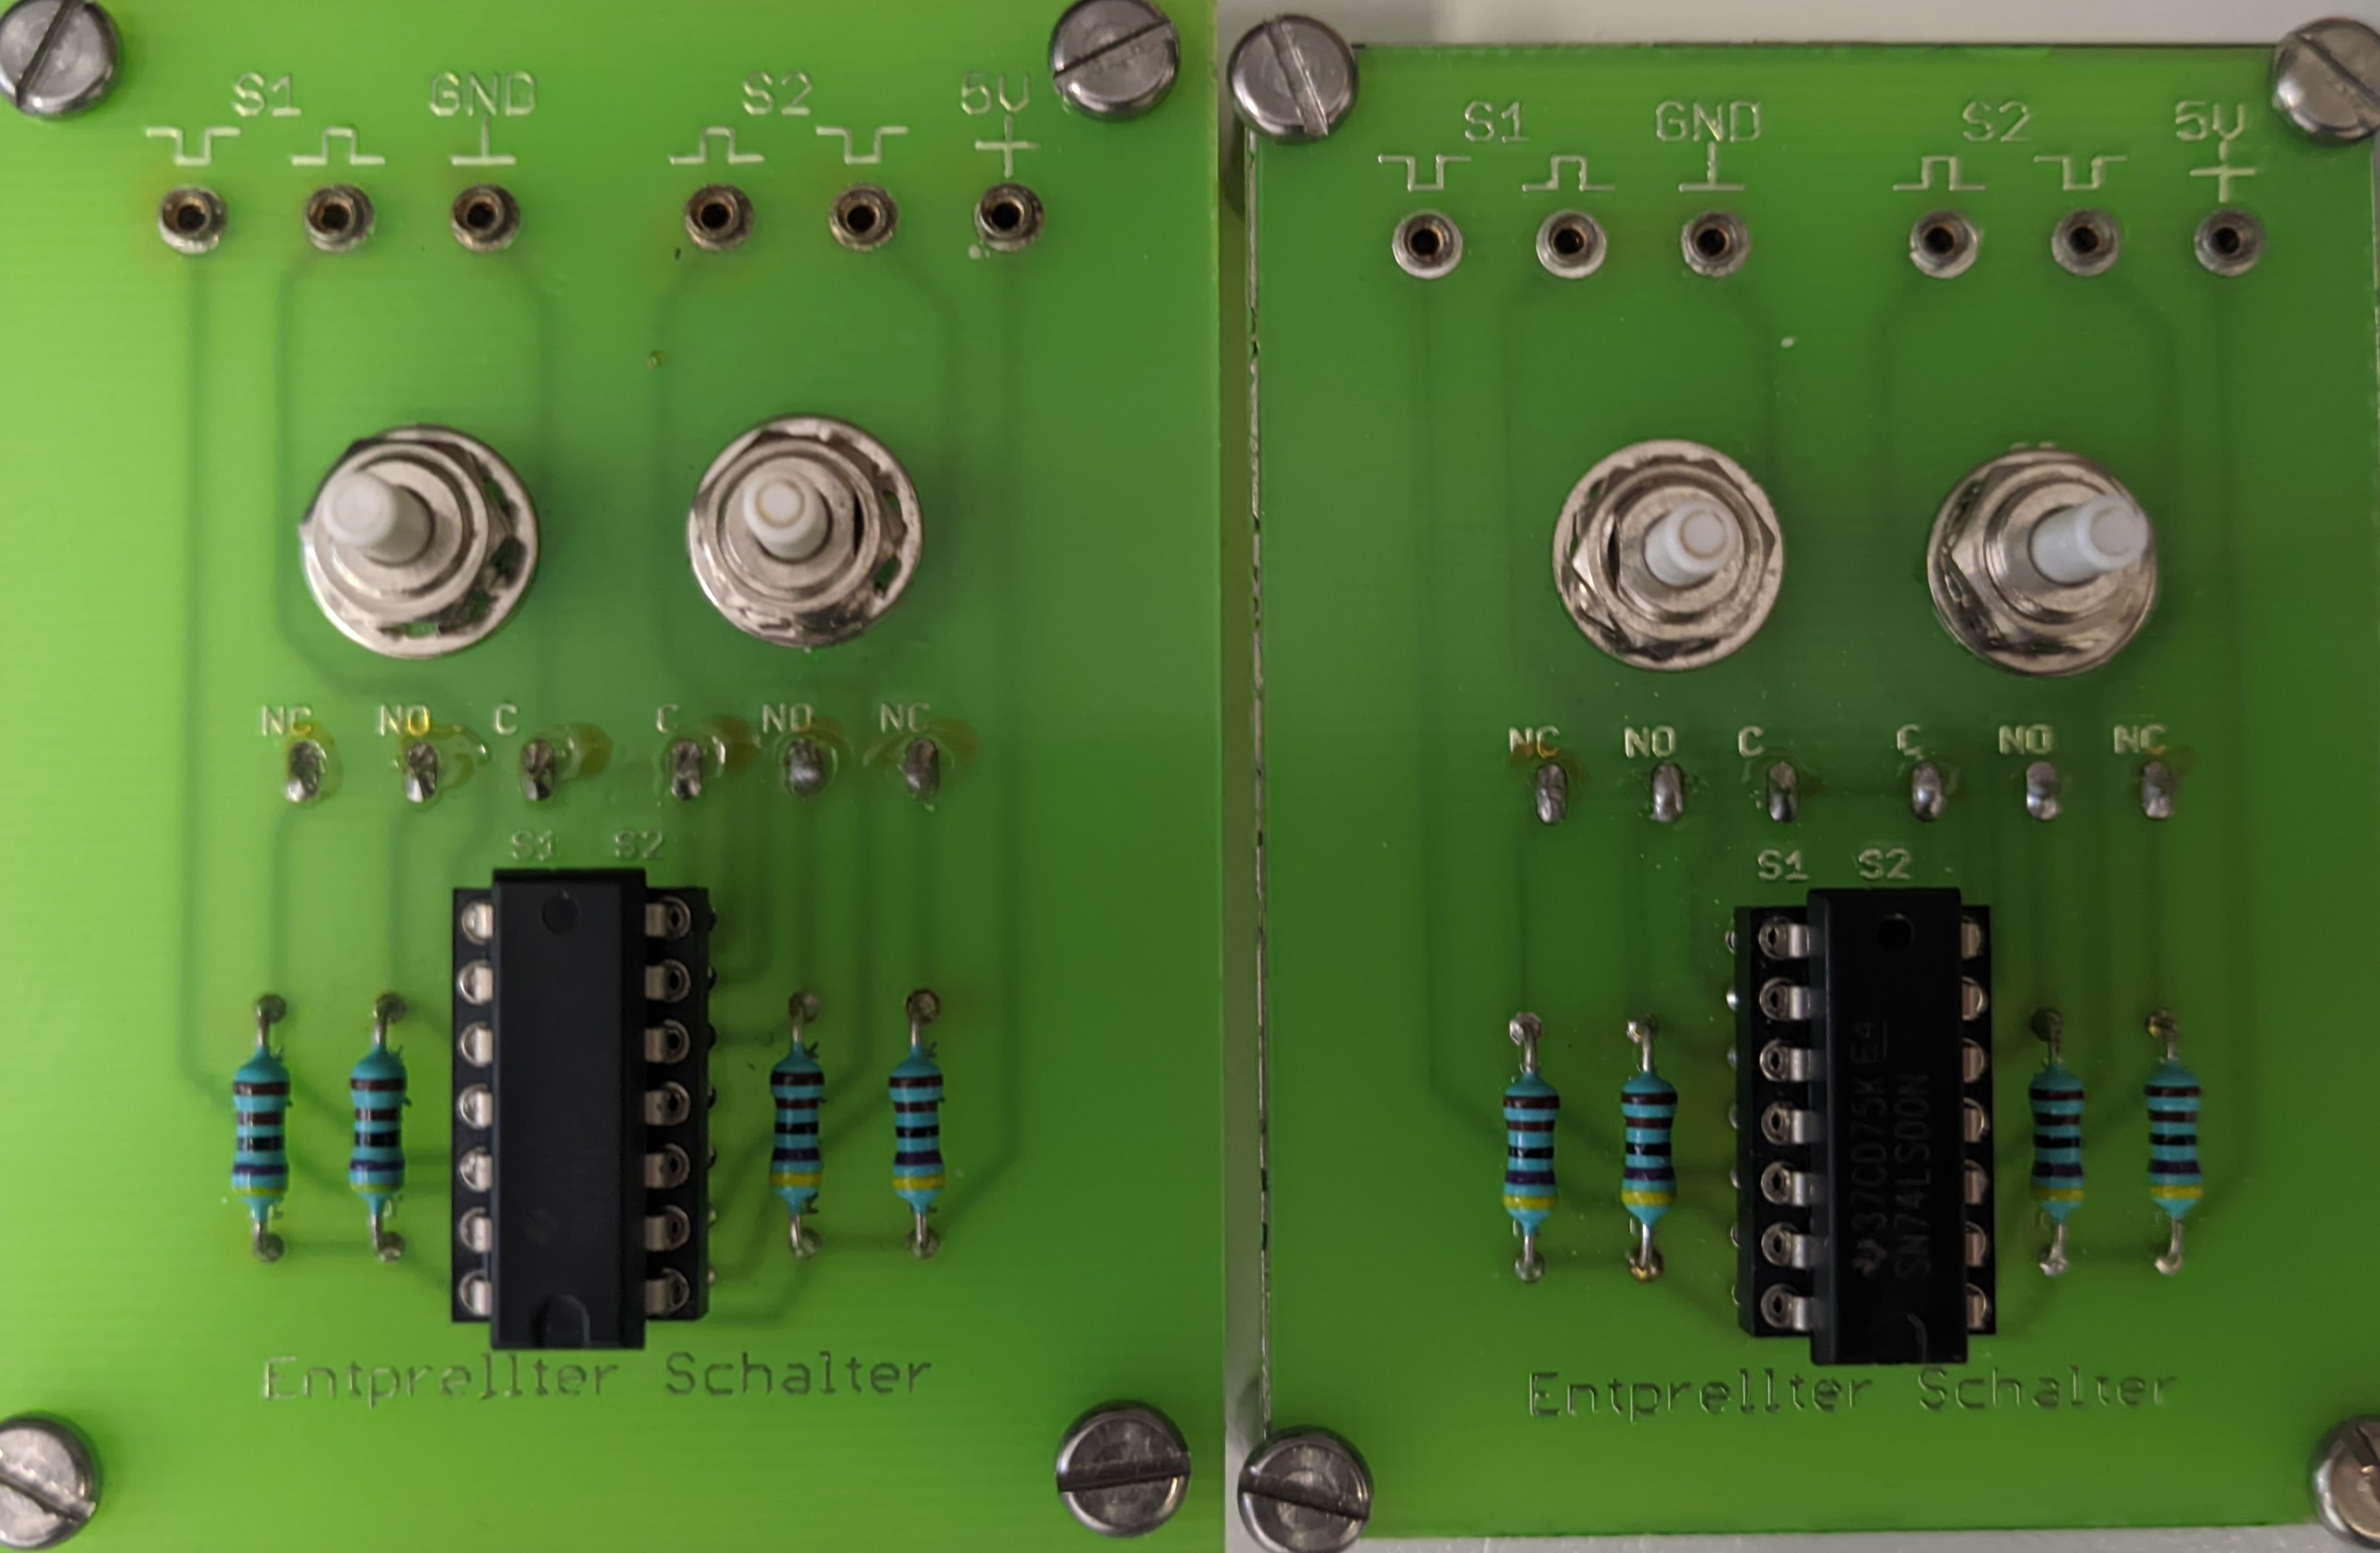
\includegraphics[width=0.95\textwidth]{./figures/messungen/schalter.jpg}
  \caption{Dies sind die zwei entprellten Schalterplatinen mit je zwei Schalter
    ($S1$,$S2$) die entweder mit Standard-\textit{HIGH} oder -\textit{LOW} verwendet
    werden können. Diese werden durch Beschalten des \textit{GND} und der \SI{5}{\volt}
    Betriebsspannung in Betrieb genommen}
  \label{fig:aufbau_schalter}
\end{figure}


\paragraph{LED Leiste}
%TODO text erklaeren wie der Leiste angesteuert wird und wo er verwendet wurde
Damit die Eingangssignale und Ausgangssignale der logischen Schaltungen
dargestellt werden können, wird eine LED-Leiste verwendet. Diese besteht aus
mehreren LEDs mit Vorwiderständen und ist in \autoref{fig:aufbau_led} dargestellt und
unterstützt bis zu 8 Aus- bzw. Eingangssignale. Die hier verwendete LED-Leiste
hat einen Common-Ground und somit werden positiven Spannungssignale direkt an den
verschiedenen Anschlüssen angelegt um die LED zum Leuchten zu bringen.

\begin{figure}[H]
  \centering
  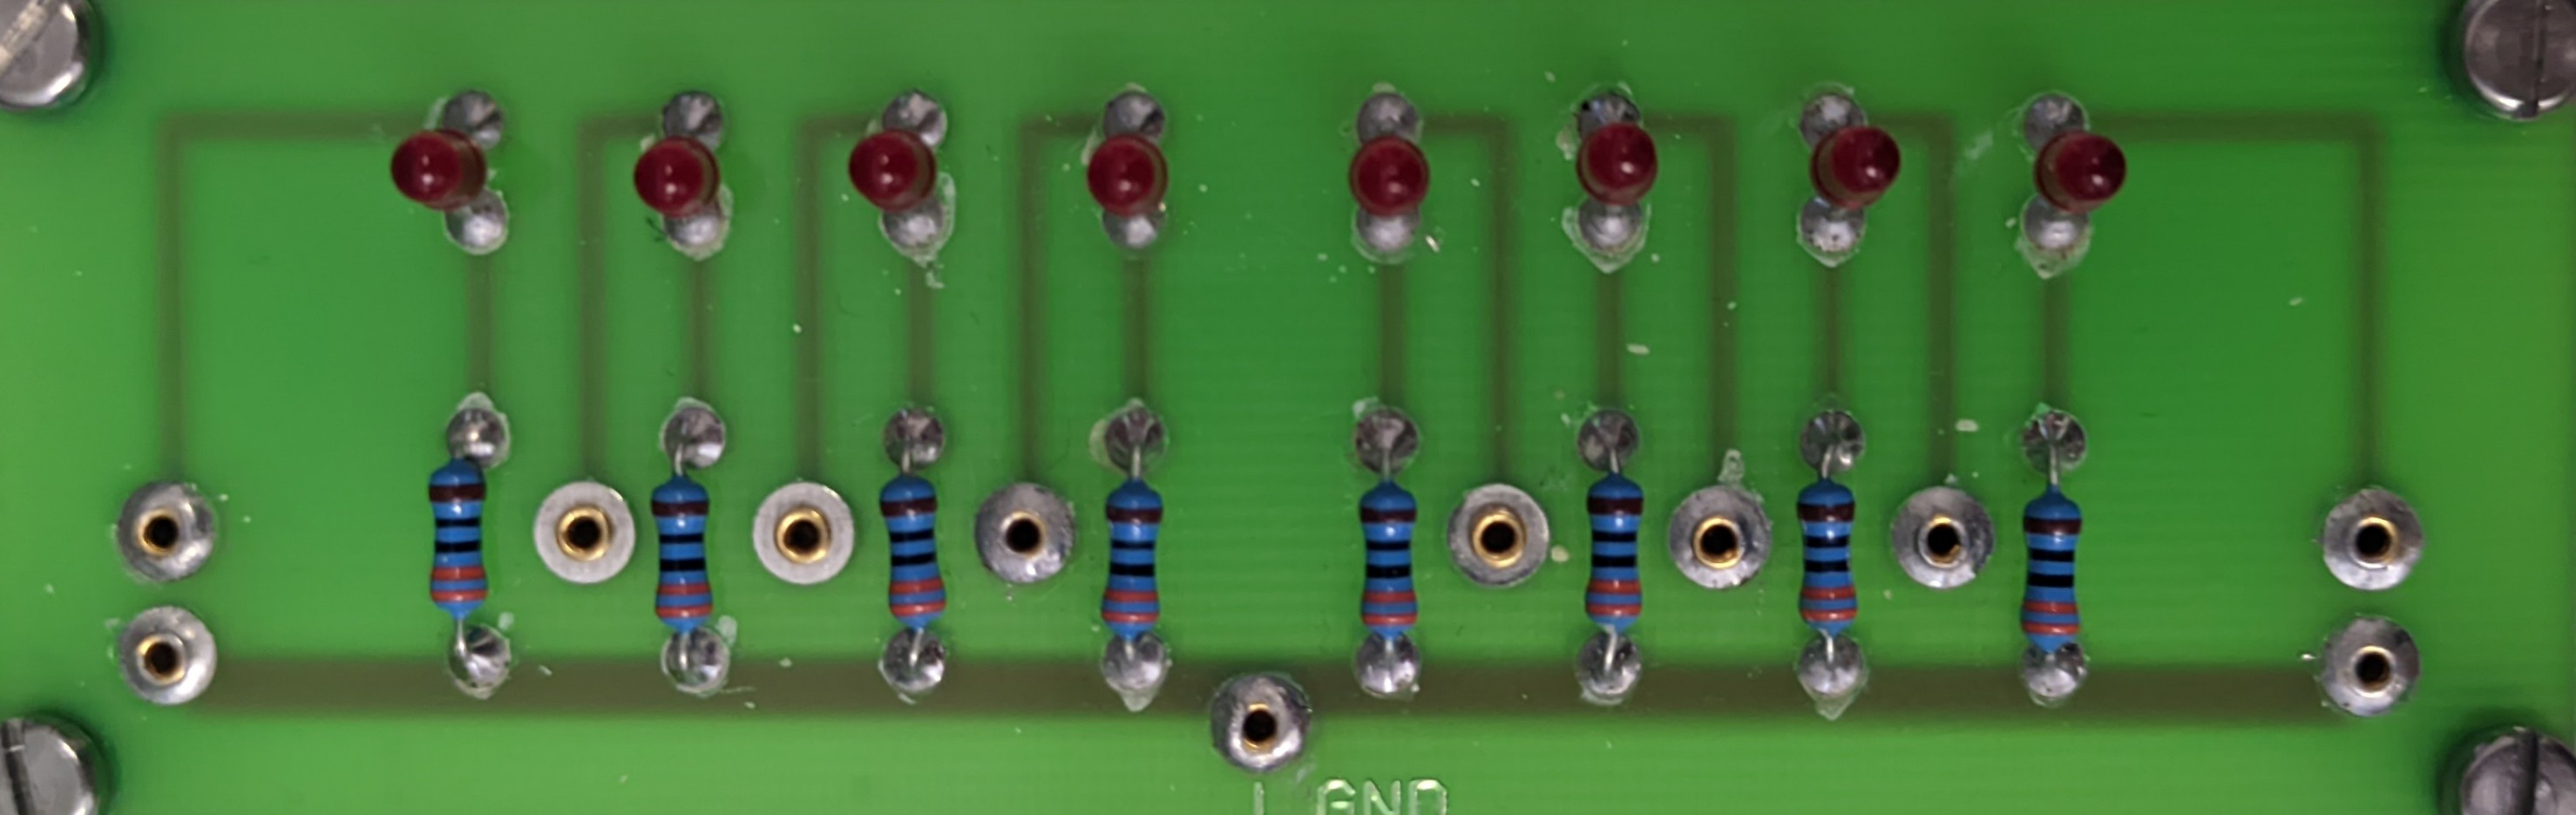
\includegraphics[width=\textwidth, height=6cm,keepaspectratio]{./figures/messungen/ledleiste.jpg}
  \caption{Dies ist die LED-Leiste, welche 8 LEDs mit je einem Vorwiderstand
  hat. Sie ist in Common-Ground-Konfiguration und wird verwendet um Signal
  anzeigen zu können.}
  \label{fig:aufbau_led}
\end{figure}

Damit die Aufnahmen der Schaltungen übersichtlich bleiben, wurde diese meistens
von den Aufnahmen weggeschnitten und dessen Funktion in der jeweiligen Grafik mittels \textit{LED} 
dargestellt oder in der Beschriftung gekennzeichnet bzw. erwähnt.

\subsection{CMOS}
% Simulation:
\subsubsection{Simulation}
% 2.1
% Die Inverter-Schaltung ist mit LTspice zu simulieren.
\paragraph{Aufbau des CMOS-Inverters}

%TODO text simulation
Die Schaltung für den CMOS-Inverter wurde gemäß \autoref{fig:sim_aufbau_inv} in LTSpice aufgebaut.
Als Betriebsspannung $U_B$ wurde eine Spannung von \SI{5}{\volt} und als Eingangsspannung $V_e$
eine Puls-Spannungsquelle mit einer Spannung von \SI{5}{\volt} (Spezifikationen nach Schaltplan) gewählt.
Bei den MOSFETs ist die richtige Beschaltung von Source, Gate und Drain zu beachten.
Weiters ist, wie gewohnt, darauf zu achten, dass nicht verwendete Anschlüsse auf Ground gelegt werden.
%TODO figure sim Aufbau
\begin{figure}[H]
  \centering
    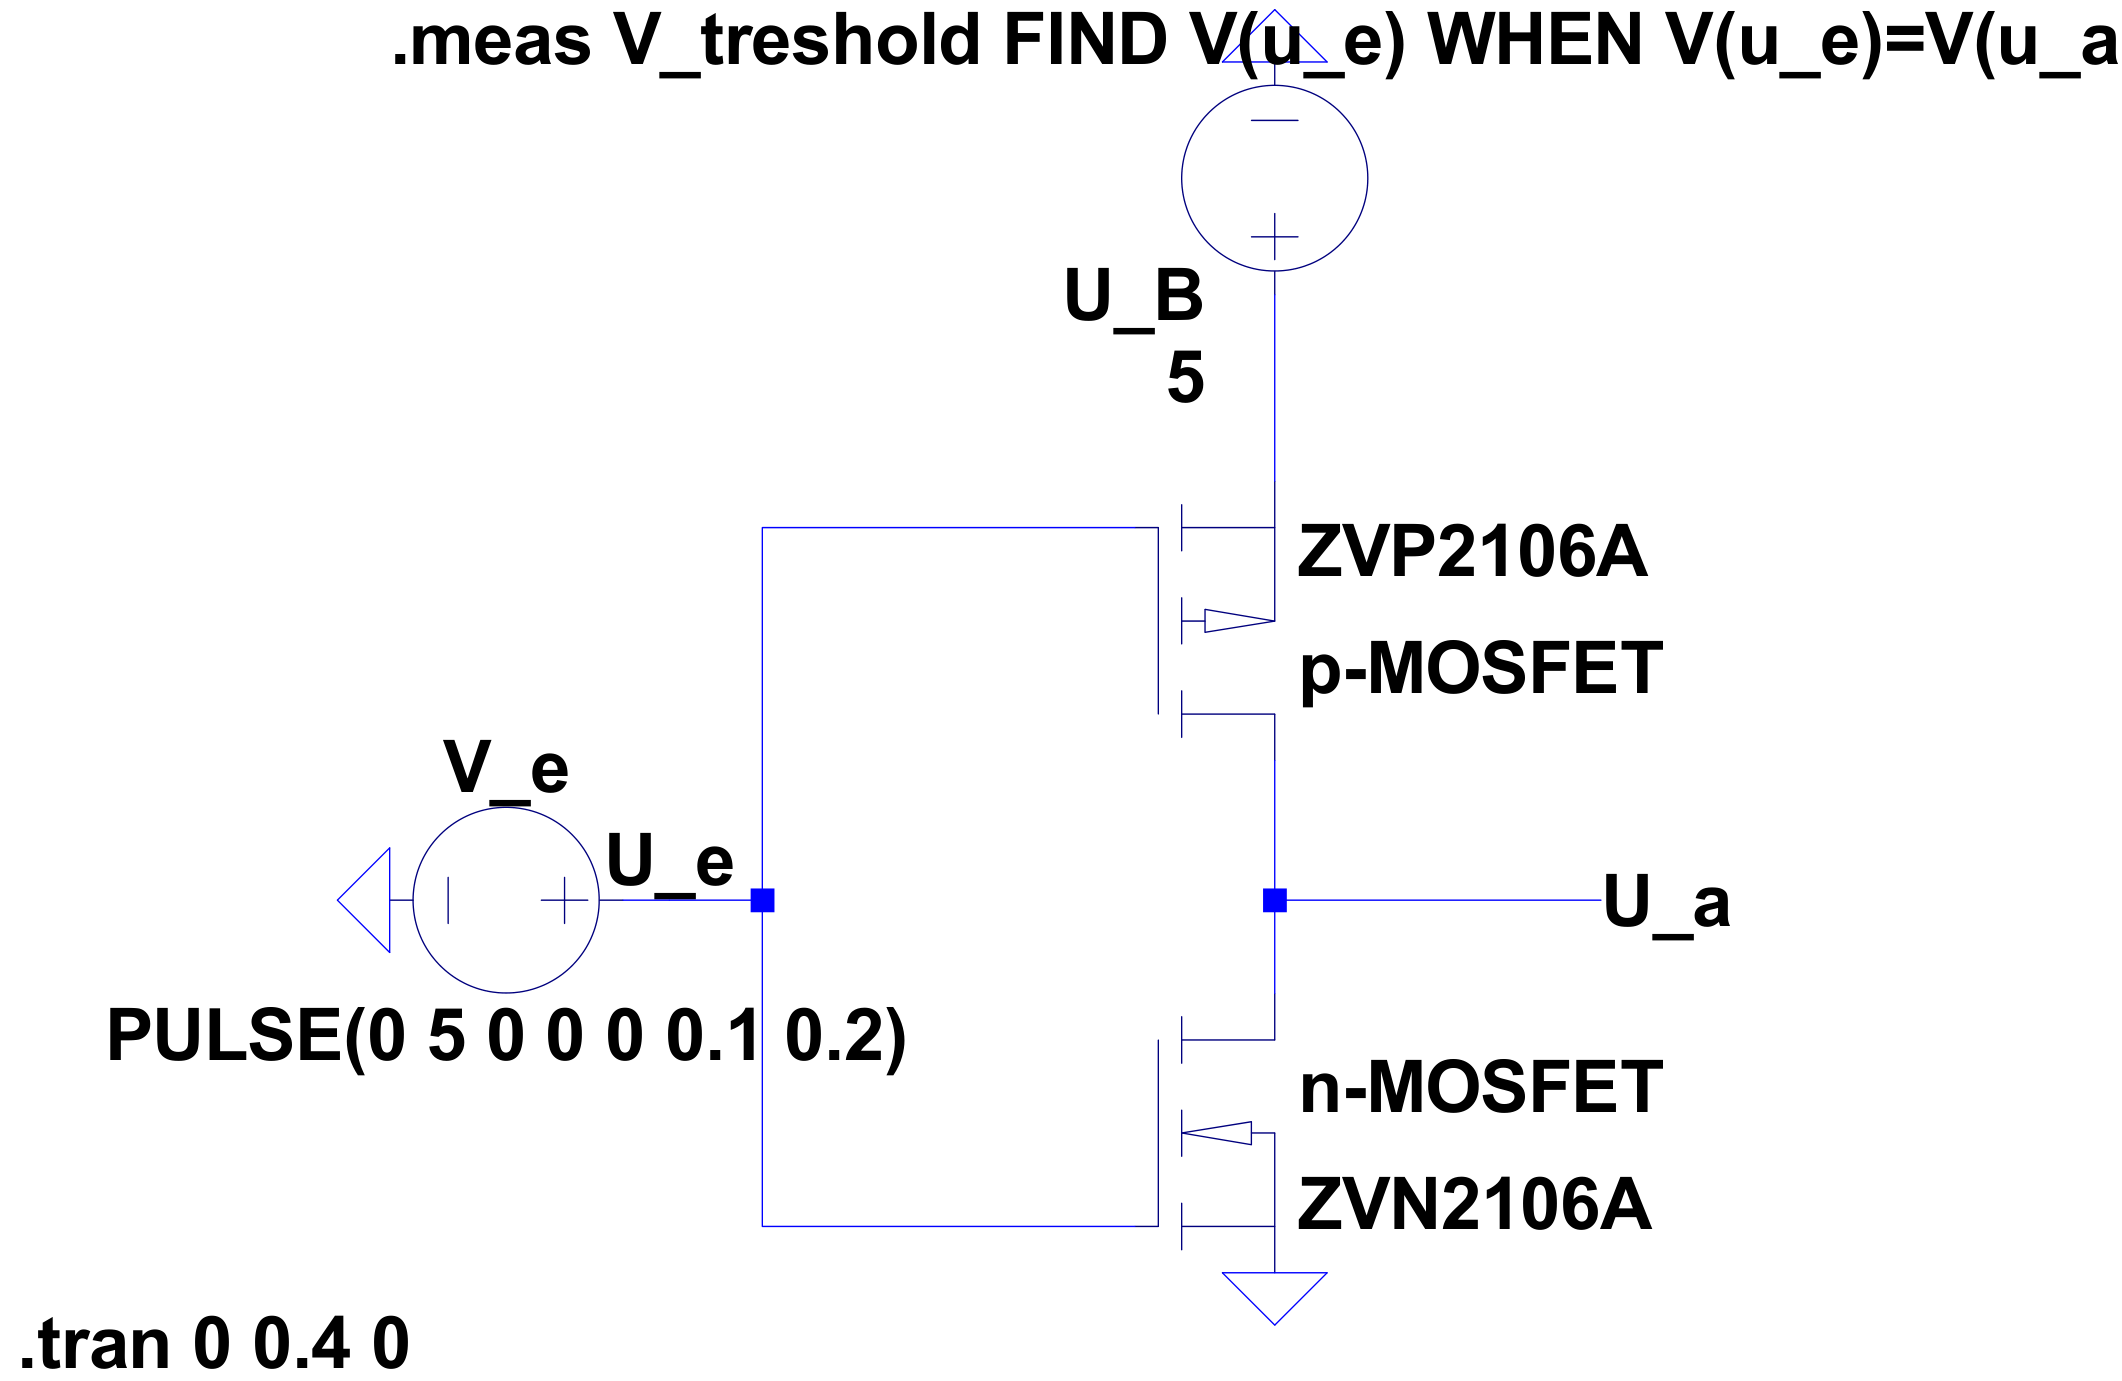
\includegraphics[width=0.95\textwidth]{./simdaten_lab/cmos/inverter/schaltung.png}
    \caption{Dieser Schaltplan zeigt, den Aufbau eines CMOS-Inverters unter
    Verwendung der Komplementären N- (\textit{ZVN2106A}) und P-MOSFETs
    (\textit{ZVP2106A}). Dabei ist $U_e$ das Eingangssignal und $U_a$ das Ausgangssignal.
    Die verwendeten Komponenten können der \autoref{tab:geraeteliste} entnommen werden.
  }
  \label{fig:sim_aufbau_inv}
\end{figure}


% Die Übertragungskennlinie
% und die Stromaufnahme sind darzustellen (PULSE-Quelle).
%TODO text messung Wie wurde simuliert wie wurde die Schwellspannung gemessen.
Daraufhin wurde eine zeitliche Transienten-Analyse der Ein- und Ausgangsspannung durchgeführt,
woraus sich \autoref{fig:sim_inv_wahrheit} ergab. Als \textit{Directive} wurde \textit{.tran 0 0.4 0} verwendet.
\begin{figure}[H]
  \centering
  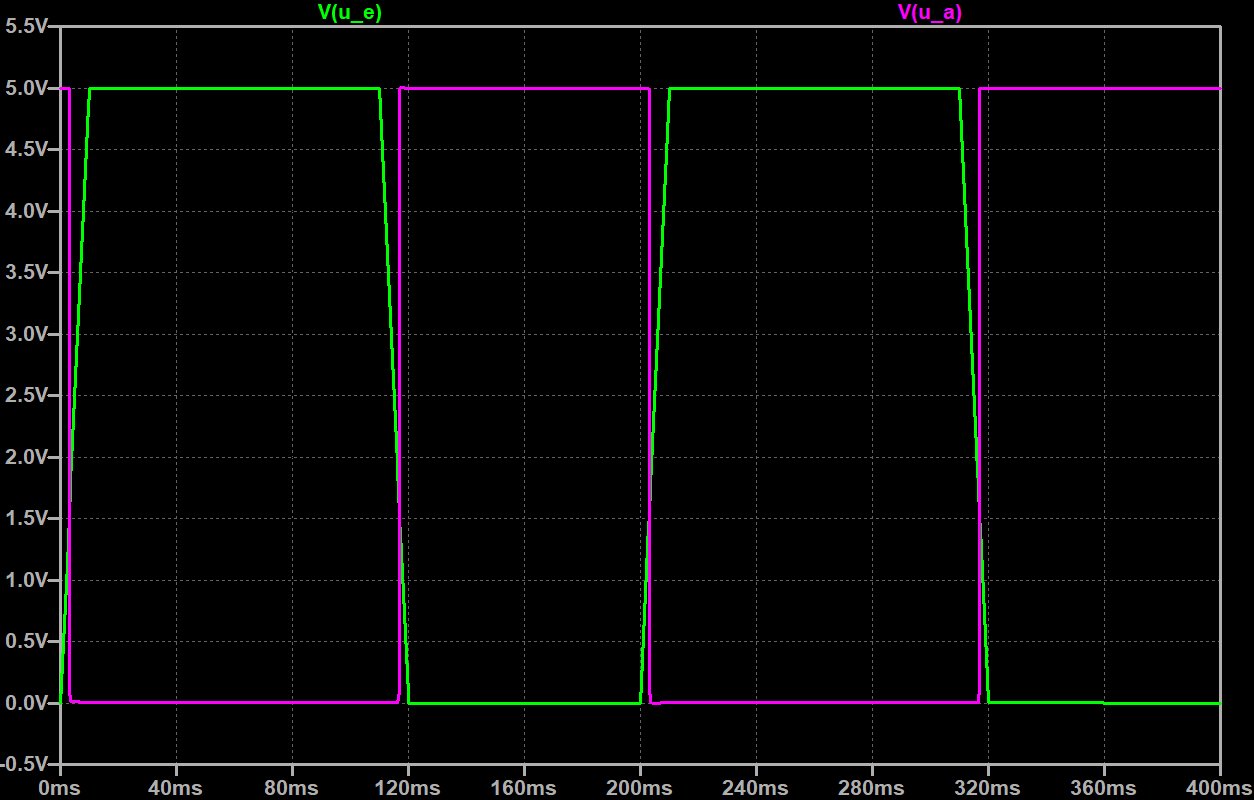
\includegraphics[width=\linewidth, height=7cm]{./simdaten_lab/cmos/inverter/kennlinie_einaus.png}
  \caption{Diese Grafik widerspiegelt das simulierte Verhalten des CMOS-NOT-Gatters (aus
    \autoref{fig:sim_aufbau_inv}) indem alle möglichen Eingangssignale
    durchgeschaltet worden sind und die Response am Ausgang aufgezeichnet
    wurde. Diese Grafik beinhaltet die simulierte Wahrheitstafel. Zudem ist
    $U_e$ das Eingangssignal und $U_a$ das Ausgangssignal. Die SPICE-Directive
    der Simulation ist \texttt{.tran 0 0.4 0}}
  \label{fig:sim_inv_wahrheit}
\end{figure}

In \autoref{fig:sim_inv_eingangsstrom} ist der Stromverlauf durch den p- respektive n-MOSFET
dargestellt. Es wurde die selbe \textit{Directive} wie für die Spannungsanalyse verwendet.

\begin{figure}[H]
  \centering
    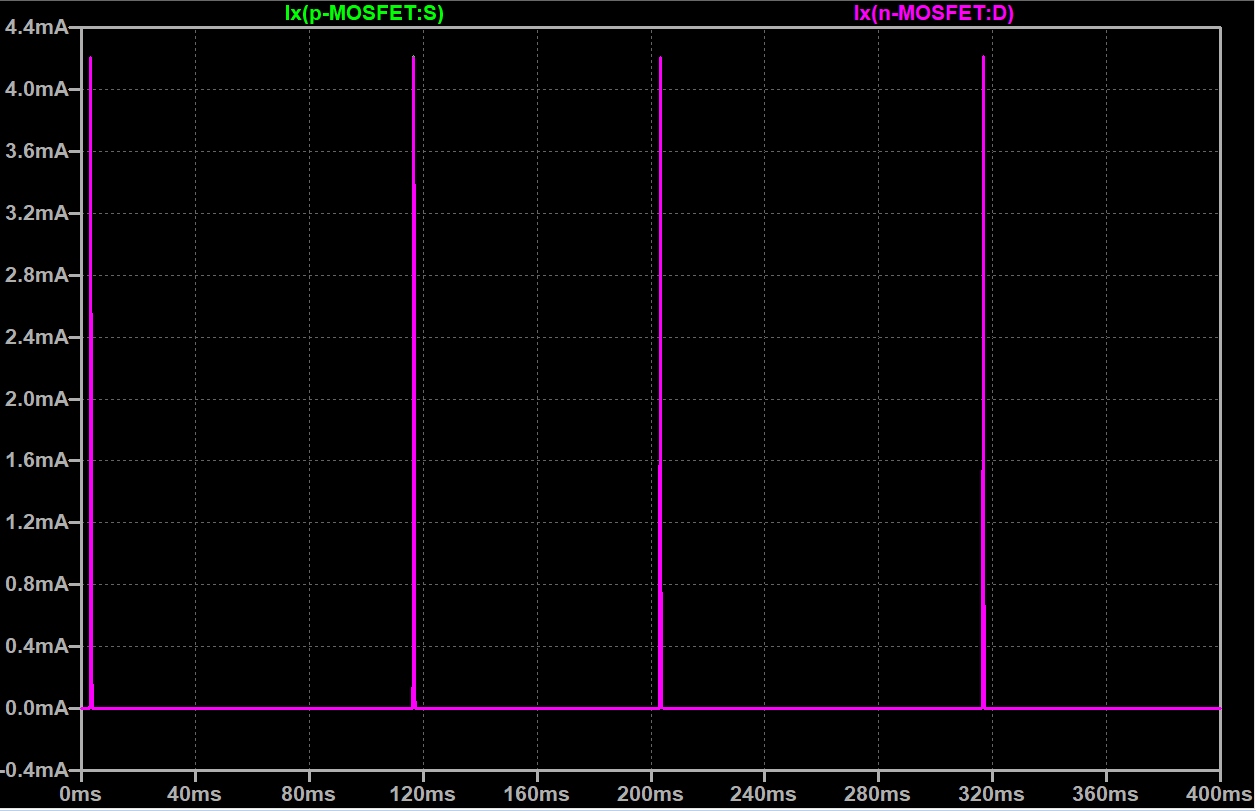
\includegraphics[width=\linewidth, height=7cm]{./simdaten_lab/cmos/inverter/strom_correct_beide.png}
    \caption{Hier sind die simulierten Gateströme des n- bzw. P-MOSFETs
    dargestellt. Die SPICE-Directive der Simulation ist \texttt{.tran 0 0.4 0}}
  \label{fig:sim_inv_eingangsstrom}
\end{figure}
%TODO figure messung
% 2.2
% Die Gate-Source Schwellspannung ist mit jener der Datenblätter zu vergleichen.

Mittels der \textit{Directive} \texttt{.meas V\_treshold FIND V(u\_e) WHEN V(u\_e)=V(u\_a)} wurde der Schnittpunkt
zwischen der Eingangs- und Ausgangsspannung bestimmt.

\begin{figure}[H]
  \centering
    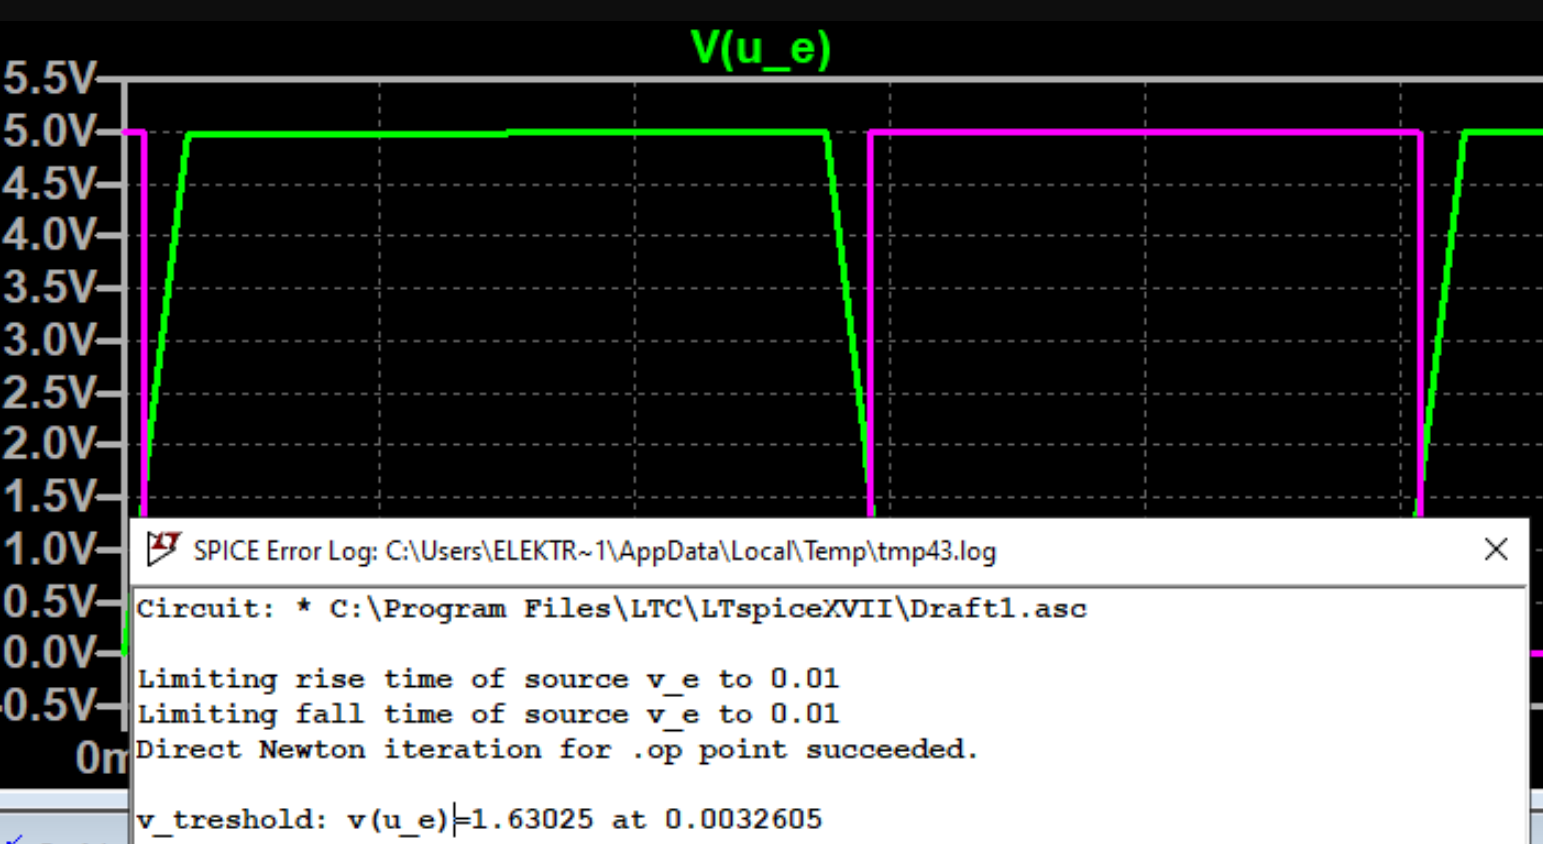
\includegraphics[width=\linewidth, height=7cm]{./simdaten_lab/cmos/inverter/treshold.png}
    \caption{Diese Grafik beinhaltet die von der Simulation errechneten
    Gate-Source Schwellspannung $V_{\mathrm{threshold}}$. Die SPICE-Directive
    der Simulation ist \texttt{.tran 0 0.4 0} und das \textit{MEASURE} Kommando
    war \texttt{.meas V\_treshold FIND V(u\_e) WHEN V(u\_e)=V(u\_a)}}
  \label{fig:sim_inv_threshold}
\end{figure}
% 2.3
% Die Schaltung des  NAND-Gatters ist mit LTspice zu simulieren. Die Ein- und
% Ausgangsspannungen sind darzustellen (PULSE-Quelle).
\paragraph{Aufbau des CMOS-NAND-Gatters}
%TODO text sim aufbau
Die Schaltung für das CMOS-NAND-Gatter wurde gemäß \autoref{fig:sim_aufbau_nand} in LTSpice aufgebaut.
Als Betriebsspannung $U_B$ wurde eine Spannung von \SI{5}{\volt} und als Eingangsspannungsquellen $V1$
und $V2$
Puls-Spannungsquellen mit einer Spannung von \SI{5}{\volt} (weitere Spezifikationen nach Schaltplan) gewählt.
Bei den verwendeten MOSFETs ist die richtige Beschaltung von Source, Gate und Drain zu beachten.
Weiters ist, wie gewohnt, darauf zu achten, dass nicht verwendete Anschlüsse auf Ground gelegt werden.
%TODO figure sim aufbau
\begin{figure}[H]
  \centering
    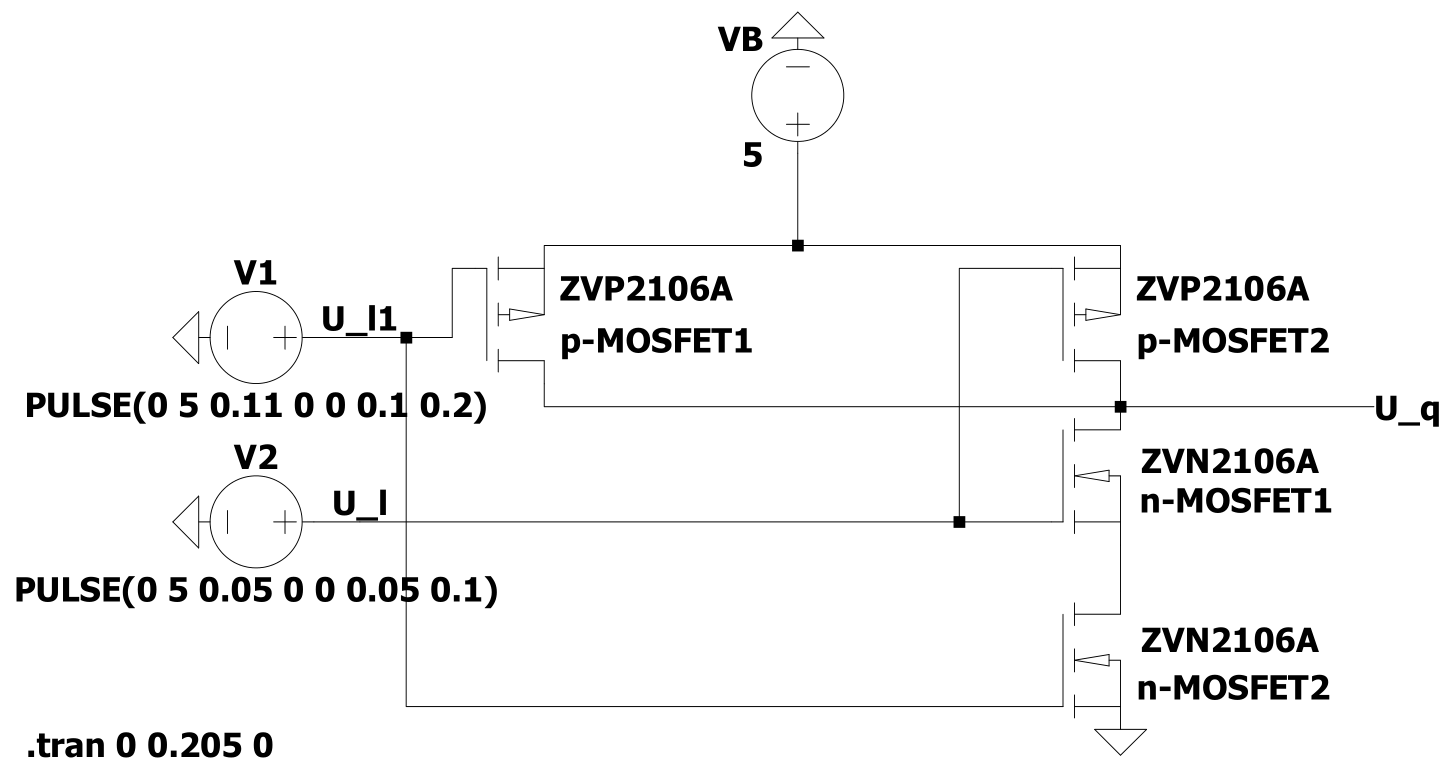
\includegraphics[width=\textwidth, height=6cm,keepaspectratio]{./simdaten_lab/cmos/nand/schaltung.png}
  \caption{Dieser Schaltplan zeigt, den Aufbau eines NAND-Gatters unter
    Verwendung der Komplementären N- (\textit{ZVN2106A}) und P-MOSFETs
    (\textit{ZVP2106A}).Dabei ist $U_l':=U_l1$, $U_l$ die logischen
  Eingangssignale und $U_q$ das Ausgangssignal.}
  \label{fig:sim_aufbau_nand}
\end{figure}

%TODO text messung Wie wurde die verschiedenen logic states geschalten
Um die möglichen Kombinationen der Eingangssignale zu erhalten, wurden
unterschiedliche Spezifikationen für die beiden Pulse-Spannungsquellen
vorgenommen; dabei wurde für $V1$ bezogen auf $V2$ eine doppelt so große
Periodendauer und Verzögerung gewählt (\textit{Directives} nach \autoref{fig:sim_aufbau_nand}).
Daraufhin wurde eine Transienten-Analyse der Spannungssignale nach der
\textit{Directive} {.tran 0 0.205 0} durchgeführt, woraus \autoref{fig:sim_nand_wahrheit} extrahiert wurde.
%TODO figure messung
\begin{figure}[H]
  \centering
    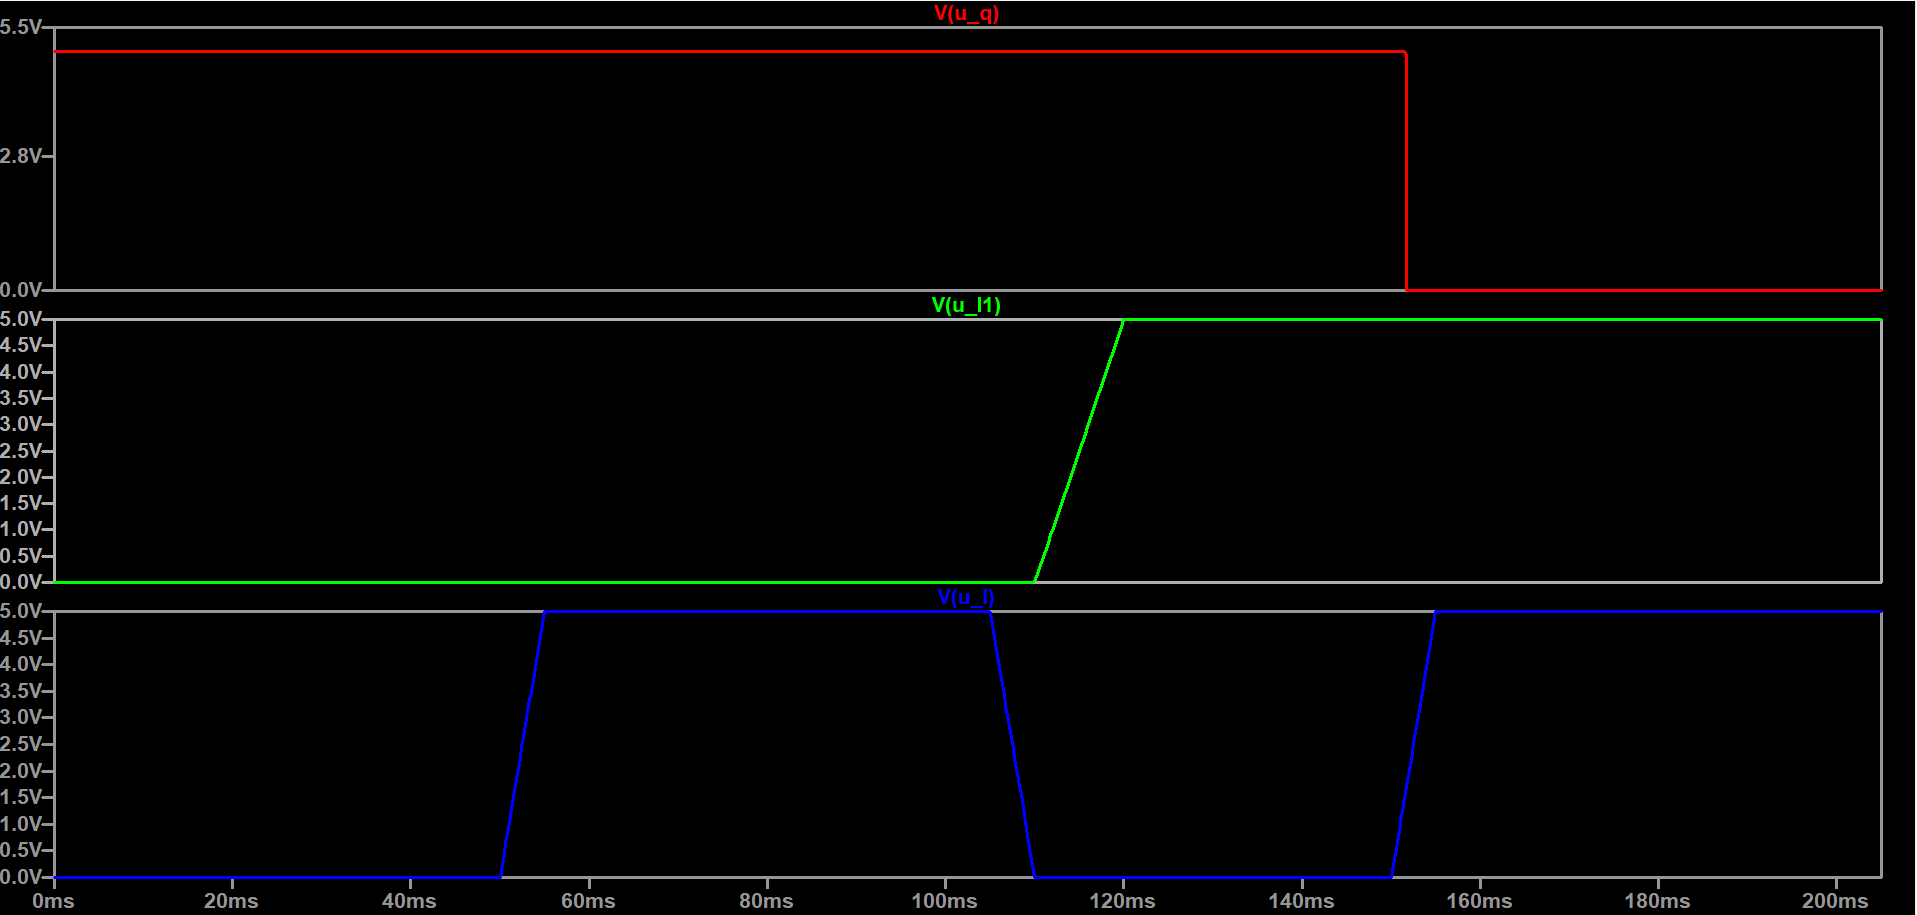
\includegraphics[width=\linewidth, height=7cm]{./simdaten_lab/cmos/nand/nand_funktion.png}
  \caption{Diese Grafik widerspiegelt das simulierte Verhalten des CMOS-NAND-Gatters (aus
    \autoref{fig:sim_aufbau_nand}) indem alle möglichen Eingangssignale
    durchgeschaltet worden sind und die Response am Ausgang aufgezeichnet
    wurde. Diese Grafik beinhaltet die simulierte Wahrheitstafel. Zudem sind
    $U_l':=U_L1,\; U_l$ die Eingangssignale und $U_q$ das Ausgangssignal. Die
    SPICE-Directive der Simulation ist \texttt{.tran 0 0.205 0}; die
  Einstellungen der Eingangssignale können der \autoref{fig:sim_aufbau_nand}
  entnommen werden}
  \label{fig:sim_nand_wahrheit}
\end{figure}

% Aufbau am Steckboard:
\subsubsection{Steckboard}
% 2.4 Der CMOS-Inverter ist auf dem Steckboard aufzubauen und seine
% Funktionalität zu prüfen. 
\paragraph{Aufbau des CMOS-Inverters}\label{sec:mess_cmos}
%TODO text
Zunächst wird der CMOS-Inverter mittels zweier MOSFETs (einem p-MOSFET \cite{ZVP2106A} und
einem n-MOSFET \cite{ZVN2106A}) wie nach dem Schaltbild (\autoref{fig:sim_aufbau_inv})
aufgebaut. Zur Visualisierung des Eingangszustands $U_l$ und des
Ausgangszustands $U_q$ wurden die LEDs der LED-Leiste parallel dazu geschaltet. Das
Eingangssignal wurde durch einen entprellten Schalter, im Standardzustand
\textit{LOW}, gegeben. Der Aufbau wird in \autoref{sec:schalter_aufbau} dargestellt. Als
Spannungsquelle wurde ein Netzgerät verwendet und auf \SI{5}{\volt}
eingestellt. 

%TODO figure
\begin{figure}[H]
  \centering
    \includegraphics[width=0.95\textwidth]{./figures/messungen/aufbauinverter.pdf}
  \caption{Dies ist der Aufbau einer CMOS-Inverter-Schaltung nach dem
  Schaltplan aus \autoref{fig:sim_aufbau_inv}, wobei $U_q$ das Ausgangssignal
  der Schaltung und $U_l$ das Eingangssignal ist. Der Zustand
  beider kann anhand einer LED in der LED-Leiste abgelesen werden.}
  \label{fig:mess_aufbau_inv}
\end{figure}


Um die Funktionstüchtigkeit des CMOS-Gatters zu überprüfen, wurde die
Wahrheitstafel des NOT-Gatters im Eingang durchgeschaltet. Die Resultate
sind in \autoref{fig:mess_wahrheitstabelle_inv} ersichtlich.
%TODO text messung
% Als  Pegelgeber wird  für  das  Steckboard  ein vorhandener  elektronisch
% entprellte  Schalter  (mit  Hilfe  eines RS-Flip-Flops)  verwendet.  Der
% Ein-  und Ausgangszustand  ist  jeweils durch  LEDs  anzuzeigen.  Die
% Funktionalität  der Schaltung ist anhand der LEDs zu zeigen.
%TODO figure messung

\begin{figure}[H]
  \centering
    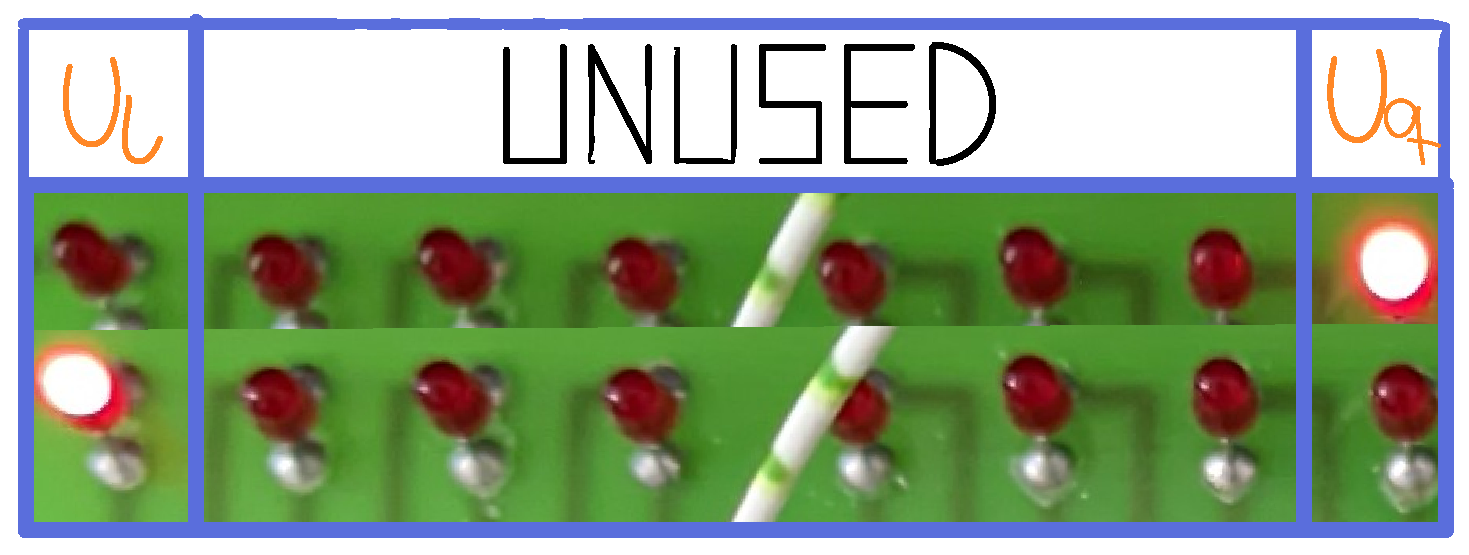
\includegraphics[width=0.95\textwidth]{./figures/messungen/WahrheitstabelleInverter.pdf}
  \caption{Diese Abbildung beinhaltet die gemessenen Eingangs- $U_l$ und
  Ausgangssignale $U_q$ der gebauten CMOS-Inverter-Schaltung. Eine leuchtende
  LED entspricht einem \textit{HIGH} Signal, eine nicht leuchtende entspricht
  \textit{LOW}} 
\label{fig:mess_wahrheitstabelle_inv}
\end{figure}


% 2.5
% Die Schaltung des  NAND-Gatters ist auf dem Steckboard aufzubauen und ihre
% Funktionalität anhand der LEDs zu zeigen.
\paragraph{Aufbau des CMOS-NAND-Gatters}
%TODO text
Nun ist CMOS-NOT Schaltung um zwei weiter MOSFETs erweitert worden, um ein
NAND-Gatter zu bauen. Dies wurde wie in \autoref{fig:sim_aufbau_nand} gemacht,
jedoch wurden, wie auch in \nameref{sec:mess_cmos}, entprellte Schalter als
Pegelgeber und die LED-Leiste zur Visualisierung der Pegel (Signale) verwendet.
Diese wurden ebenfalls an den geeigneten Stellen angeschlossen, wie diese genau
angeschlossen wurden ist der \autoref{fig:mess_aufbau_nand} entnehmbar.

%TODO figure
\begin{figure}[H]
  \centering
    \includegraphics[width=0.95\textwidth]{./figures/messungen/aufbaunand.pdf}
  \caption{Dies ist der Aufbau eines CMOS-NAND-Gatters nach dem Schaltplan aus
  \autoref{fig:sim_aufbau_nand}}
  \label{fig:mess_aufbau_nand}
\end{figure}

%TODO text messung
Um die Funktionstüchtigkeit des CMOS-Gatters zu überprüfen wurde die
Wahrheitstafel des NAND-Gatters in den zwei Eingängen ($U_l$ $U_l'$) durch
geschaltet die gemessenen Werte sind in \autoref{fig:mess_wahrheitstabelle_nand}
ersichtlich.


%TODO figure messung
\begin{figure}[H]
  \centering
    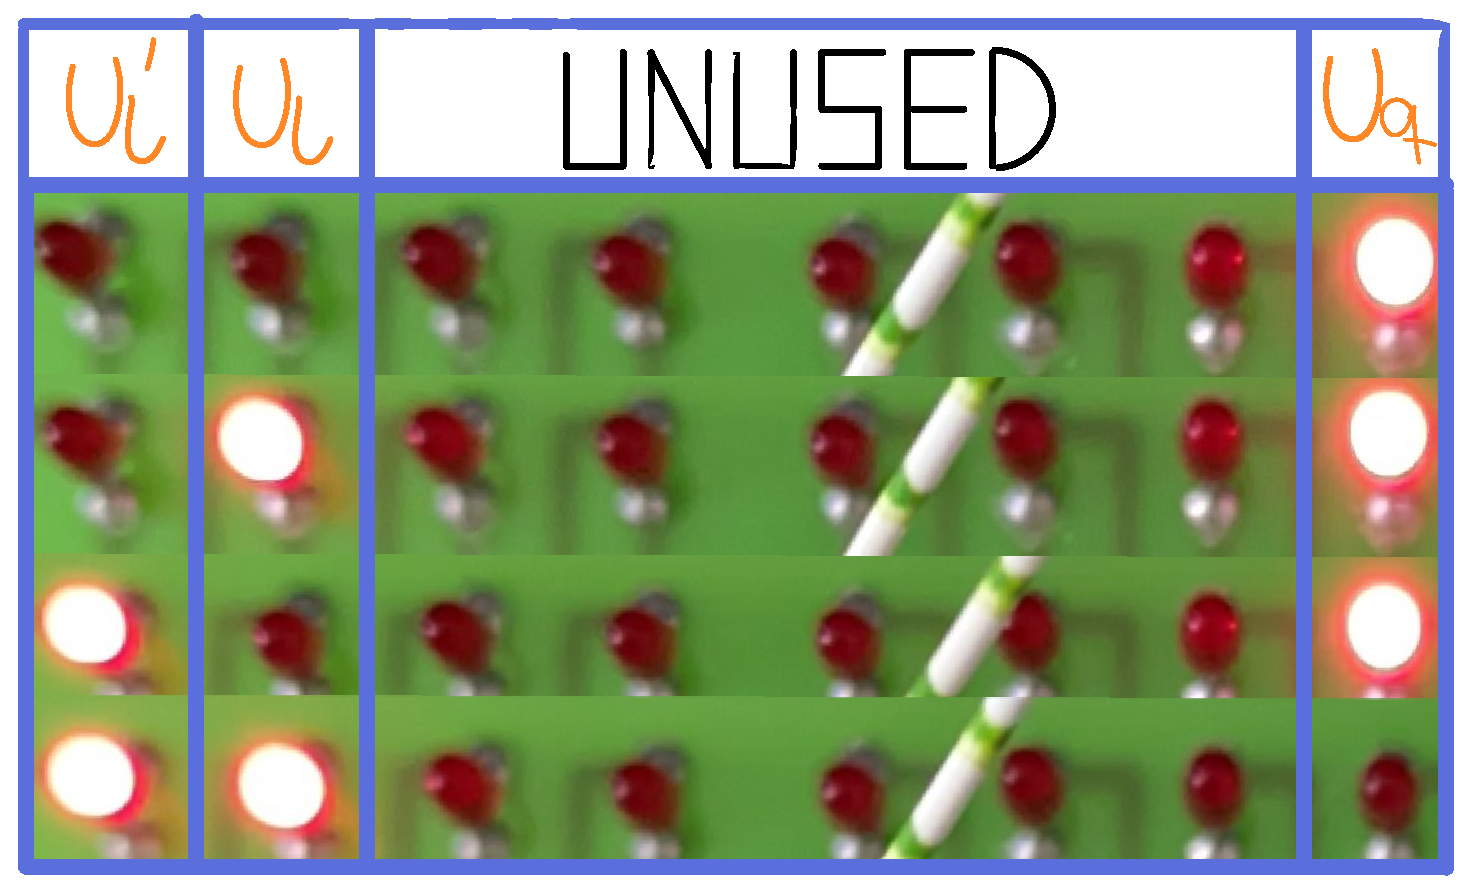
\includegraphics[width=0.95\textwidth]{./figures/messungen/WahrheitstabelleNAND.pdf}
  \caption{Diese Abbildung beinhaltet die gemessenen Eingangs- $U_l$,$U_l'$ und
  Ausgangssignale $U_q$ der gebauten CMOS-NAND-Schaltung. Eine leuchtende
  LED entspricht einem \textit{HIGH} Signal und nicht leuchtend entspricht
  \textit{LOW}}
  \label{fig:mess_wahrheitstabelle_nand}
\end{figure}

% 2.6
% Die Ergebnisse sind zu protokollieren und diskutieren.

\subsection{Schaltungssynthese}
% Simulation:
% 2.1 Die Schaltung ist mit LTspice zu simulieren.
\subsubsection{Simulation}

%TODO text sim aufbau

%TODO figure sim aufbau
\begin{figure}[H]
  \centering
    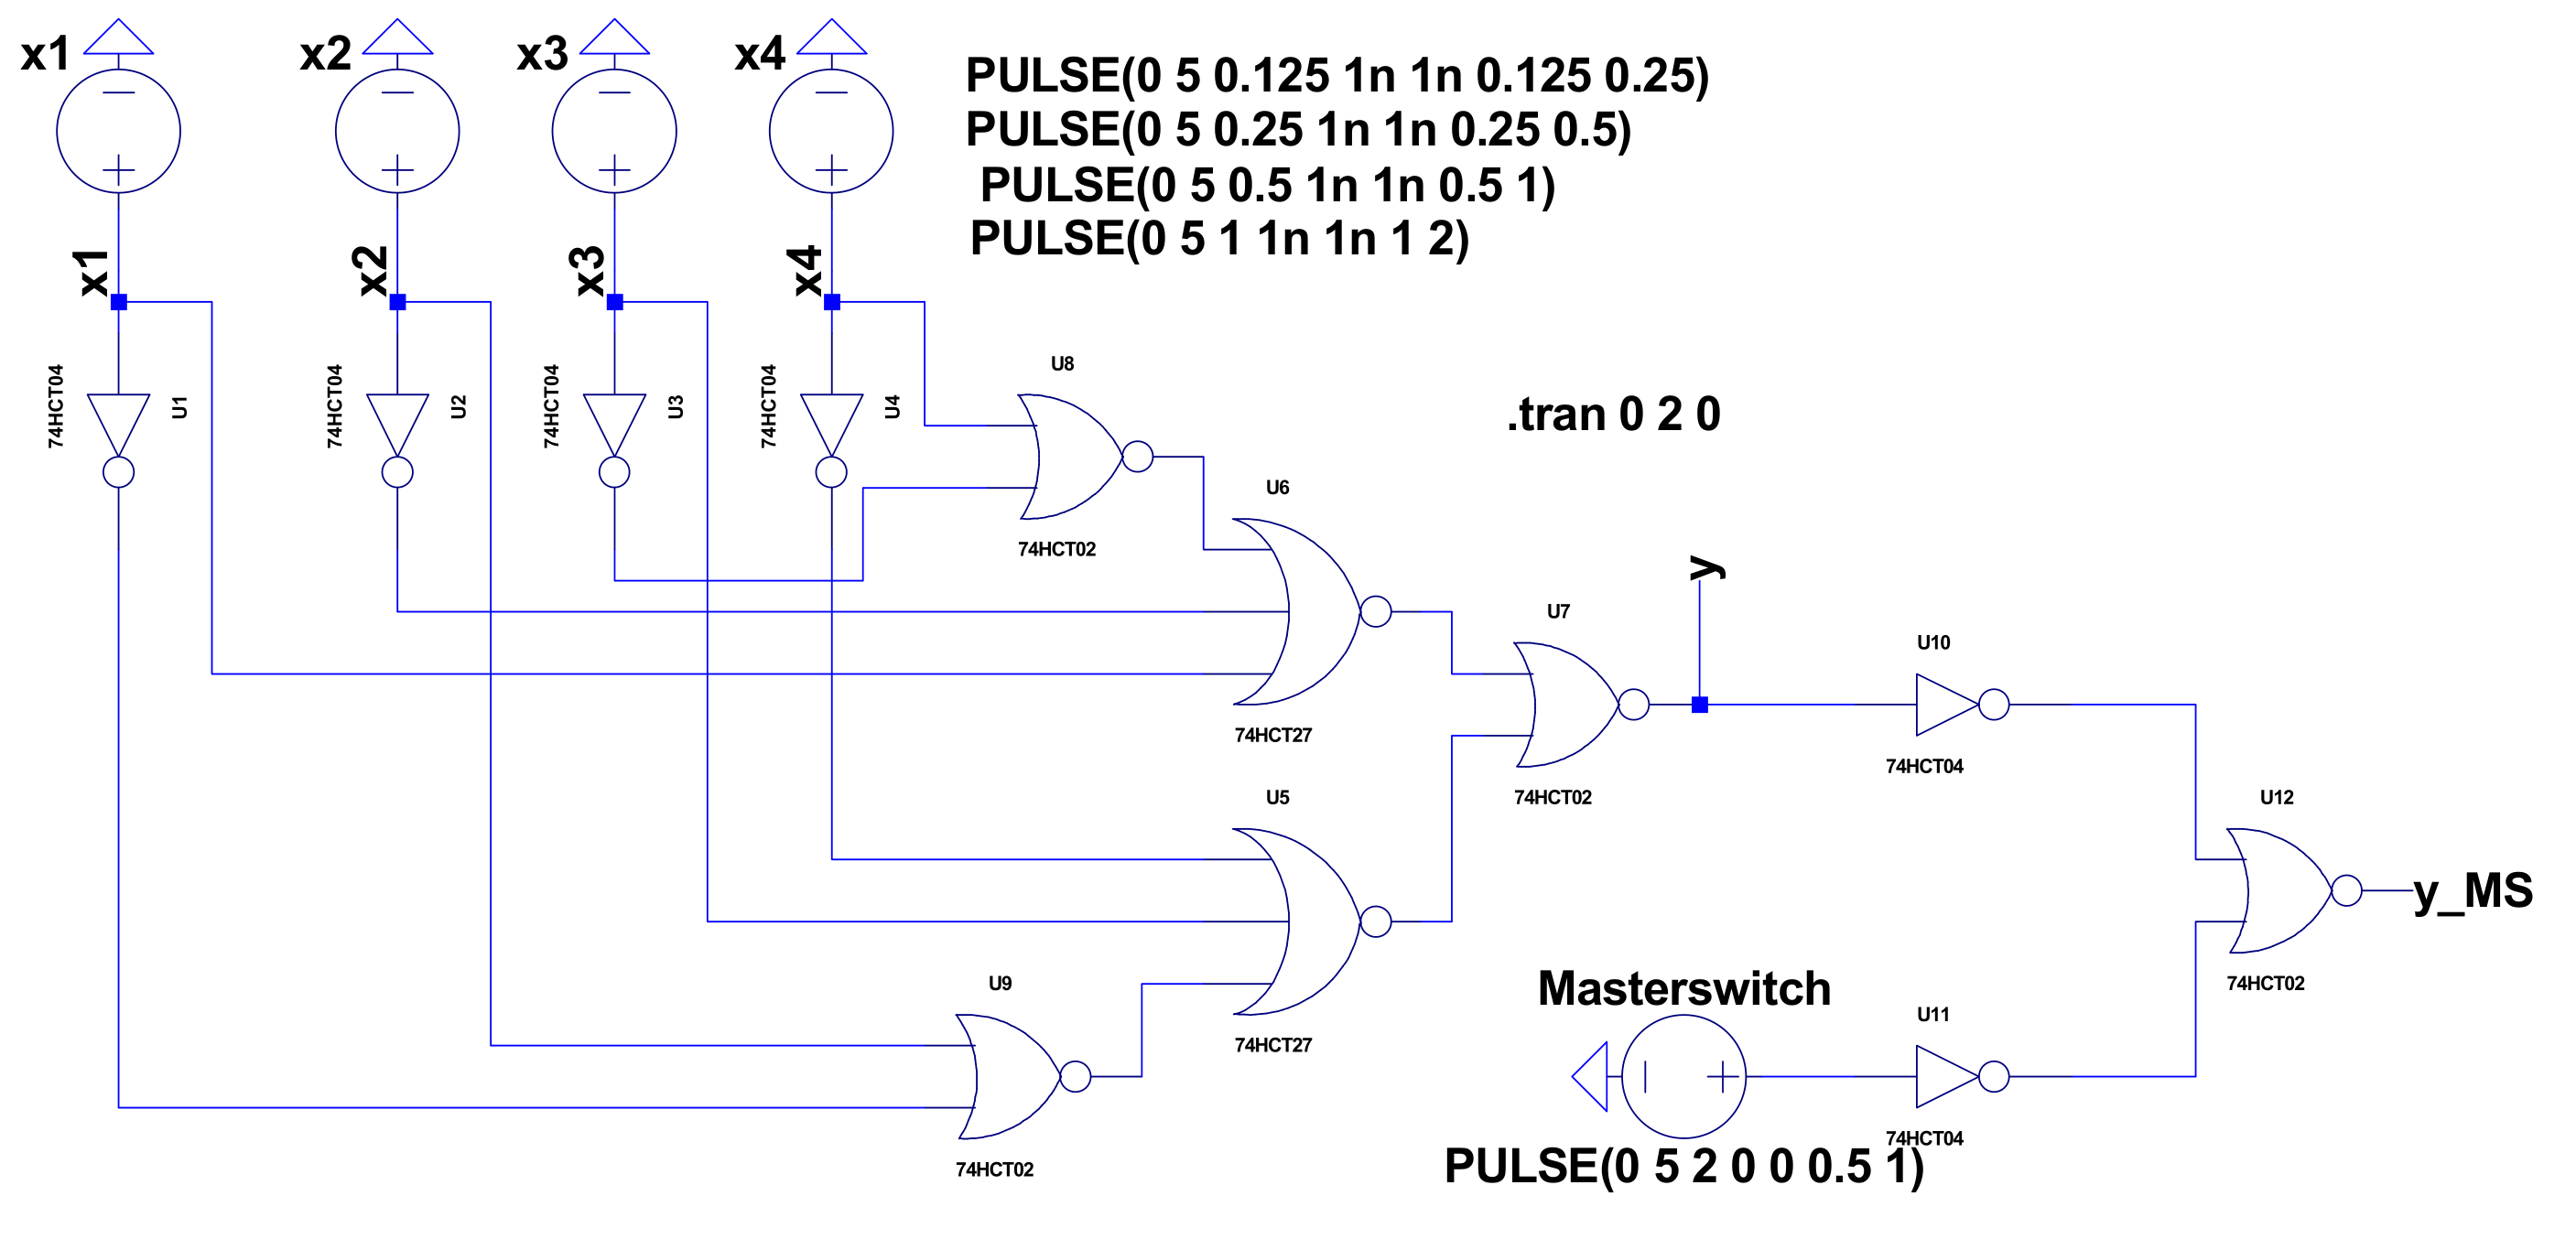
\includegraphics[width=0.95\textwidth]{./simdaten_lab/logic/schaltung.png}
    \caption{Dies Schaltung entspricht der in der
    \nameref{sec:Aufgabenstellung} aufgetragenen und in
  \nameref{sec:Vorbereitung} entworfenen Einbruchsicherungsschaltung. Hier
  entspricht $x1$ dem Fensterscheiben-Vibrationsfühler, $x2$ dem
  Tür-Kontaktfühler, $x3$ der Ultraschall-Raumüberwachung und $x4$ der
  Infrarot-Lichtschranke. Zudem ist hier auch der \textit{Master-Switch}
ersichtlich. Die verwendeten Komponenten können der \autoref{tab:geraeteliste}
entnommen werden.}
  \label{fig:sim_aufbau_alarm}
\end{figure}

% Die Eingangsspannungen, für die geeignete Perioden zu definieren sind, sowie
% die Ausgangsspannung sind darzustellen.
%TODO text messung Wie wurde die verschiedenen logic states geschalten

%TODO figure messung
\begin{figure}[H]
  \centering
    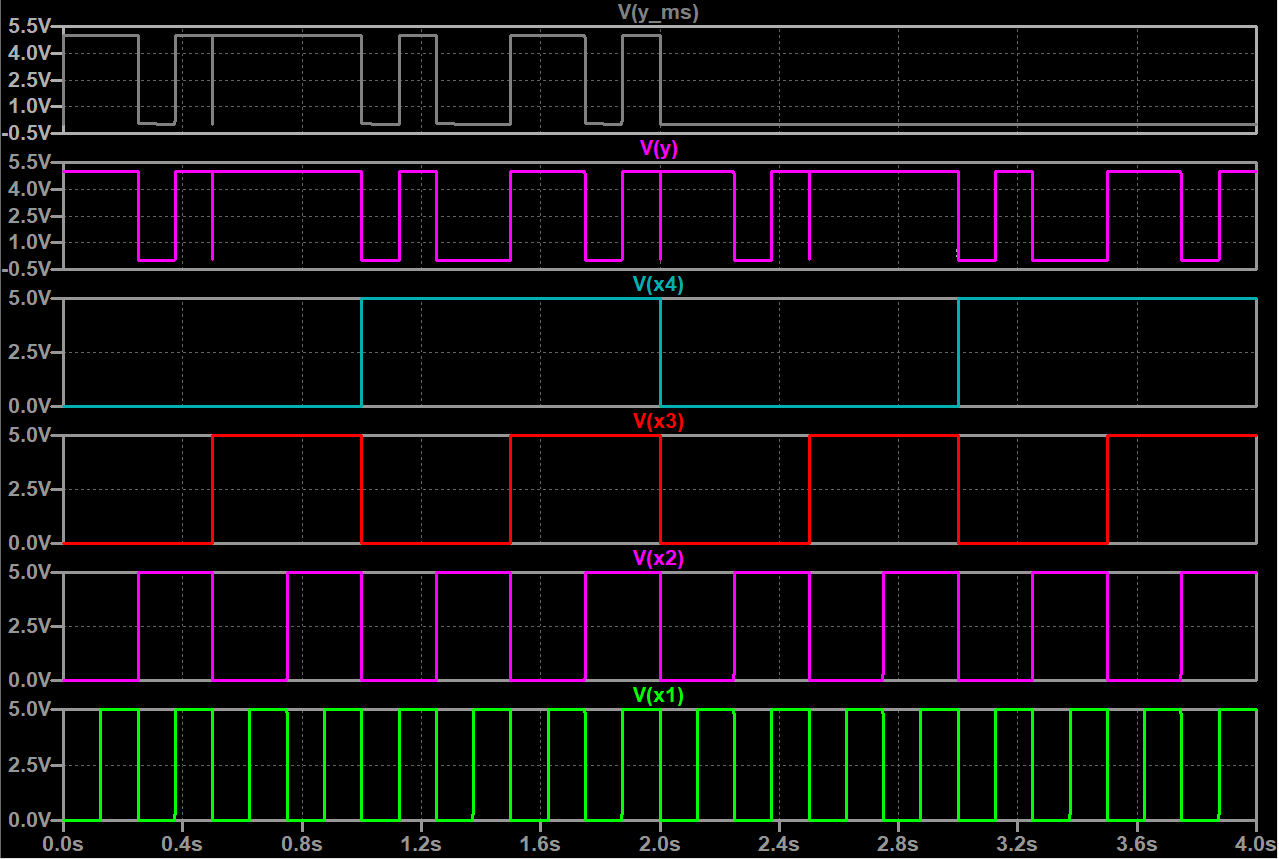
\includegraphics[width=0.95\textwidth]{./simdaten_lab/logic/master_verlauf.png}
  \caption{Diese Grafik widerspiegelt das Verhalten der
    Einbruchsicherungsschaltung (aus \autoref{fig:sim_aufbau_alarm}) indem alle
    möglichen Eingangssignale durchgeschaltet worden sind und die Response am
    Ausgang aufgezeichnet wurde. Diese Grafik beinhaltet die simulierte
    Wahrheitstafel. Zudem sind $x1$, $x2$, $x3$, $x4$ \&
    der \textit{Master-Switch} die Eingangssignale und $y$ das Ausgangssignal. Die
    SPICE-Directive der Simulation ist \texttt{.tran 0 4 0}; die
    Einstellungen der Eingangssignale können der \autoref{fig:sim_aufbau_alarm}
  entnommen werden}
  \label{fig:sim_alarm_wahrheit}
\end{figure}


% Aufbau am Steckboard:
\subsubsection{Steckboard}
Wie in der \nameref{sec:Aufgabenstellung} gesagt wurde galt es eine Schaltung
zu designen, welche durch anschlagen zweier Sensoren einen Alarm auslösen
sollte. Diese Schaltung wurde um die Fehlerquellen zu reduzieren jedoch aus der
Musterlösung entnommen und nicht die Eigengestaltete verwendet. Die vier
Eingangsgrößen ($x1$, $x2$, $x3$, $x4$) wurden durch vier entprellte
Schalter realisiert. Dabei sind $x1$ \& $x3$ im Standard \textit{LOW} und
$x2$ \& $x4$ Standard \textit{HIGH} Betrieb geschaltet worden. Damit die
Alarmanlage bei Signalunterbrechung $x2$ \& $x4$ und einer Signal bei $x1$
\& $x3$ anschlagt. Das Design der Schaltung der \nameref{sec:Aufgabenstellung}
entnommen werden.

%TODO figure
\begin{figure}[H]
  \centering
    \includegraphics[width=0.95\textwidth]{./figures/messungen/aufbaualarm.png}
  \caption{Dies ist der Aufbau der Einbruchsicherungsschaltung nach dem
  Schaltplan aus \autoref{fig:sim_aufbau_alarm}}
  \label{fig:mess_aufbau_alarm}
\end{figure}

% 2.2
% Die Schaltung ist am Steckboard aufzubauen und ihre Funktionalität an Hand der 
% Wahrheitstafel zu zeigen. Als Pegelgeber werden für das Steckboard vorhandene 
% elektronisch entprellte Schalter verwendet. Die logischen Zustände von x1, x2, x3, 
% x4 und y, sowie des Master-Switch, sind durch LEDs anzuzeigen.
%TODO text messung
Um die Funktionstüchtigkeit der Einbruchsicherungsschaltung zu überprüfen
sind alle Kombinationen der vier Eingangsgrößen ($x_1$, $x_2$, $x_3$, $x_4$)
gemessen worden. Somit konnte die Wahrheitstafel der Schaltung erstellt werden,
die gemessenen Werte sind in \autoref{fig:mess_wahrheitstabelle_alarm}
ersichtlich.

%TODO figure messung
\begin{figure}[H]
  \centering
    \includegraphics[width=0.95\textwidth,height=15cm]{./figures/messungen/WahrheitstabelleAlarm.pdf}
  \caption{Diese Abbildung beinhaltet die gemessenen logischen Zustände der
    Ein- $x1$, $x2$, $x3$, $x4$ und Ausgänge $y$ der gebauten
    Einbruchsicherungsschaltung. Eine leuchtende LED entspricht einem
    \textit{HIGH} Signal und nicht leuchtend entspricht \textit{LOW}}
  \label{fig:mess_wahrheitstabelle_alarm}
\end{figure}

Für die Untersuchung des Master-Switches im ausgeschalteten Zustand wurden die
eine zuvor wahre Eingangssignalkombination geschaltet und geschaut ob diese
nicht die Alarmanlage anschlagen lässt. Da die Schaltung zuvor, wie in
\autoref{fig:mess_wahrheitstabelle_alarm} ersichtlich, funktionierte ist
dadurch die Funktionstüchtigkeit des Master-Switches gezeigt.

% 2.3
% Die Ergebnisse sind zu protokollieren und zu diskutieren.

% zu 4: Auswertung siehe EPM Skript nur Besprechung von Umformungen und 
% Sachen die man mit den Messungen machen muss damit man Conclusion und Wissen 
% gewinnen kann.
% Entsprechend der in Punkt 2. angegebenen Beziehungen (Formeln) ist aus den
% Messergebnissen in Punkt 5. das in Punkt 1. formulierte Endergebnis zu
% berechnen. Oft ist eine Ermittlung des Endergebnisses aus einer grafischen
% Darstellung bzw. eine grafische Veranschaulichung zweckmaßig. Dabei kann
% die Verwendung von Millimeterpapier oder Computerprogrammen hilfreich sein.
% Wenn eine Bearbeitung der Daten auf dem Computer erfolgt, sollte bei der
% Darstellung der Graphen eine sinnvolle Skalenteilung des Koordinatensystems
% gemacht werden. Die Unsicherheitsbetrachtung f ̈ur die angegebenen Messwerte,
% sowie fur Zwischen- und Endergebnisse ist in diesem Abschnitt
% nachvollziehbar zu beschreiben. Dabei ist nach Kapitel 1 vorzugehen und
% insbesondere auf die Klassifizierung der Unsicherheit (Typ-A/B) und die
% Unsicherheitsfortpflanzung einzugehen.
\section{Auswertung}\label{sec:Auswertung}


% zu 5: Diskussion und Zusammenfassung
% In der Zusammenfassung stehen noch einmal die wichtigsten Messergebnisse, wobei auf Tabellen und
% Abbildungen nur verwiesen werden soll. Die Ergebnisse sind auch zu diskutieren. Insbesondere müssen
% Abweichungen zwischen Simulation und praktischer Durchführung diskutiert werden.
\section{Diskussion und Zusammenfassung}\label{sec:Diskussion} 
\subsection{Diskussion}
In \autoref{fig:sim} von der Simulation und \autoref{}, das die LEDs vom Steckbrett zeigt,
ist das Verhalten eines CMOS-Inverters gut zu erkennen; dabei wird das Signal
am Ausgang relativ zu jenem am Eingang negiert.
Weiters ist anhand von \autoref{} aus der Simulation ersichtlich, dass
der Schaltvorgang in CMOS endlich schnell erfolgt. Dabei ist ein deutliches
Maximum des Stroms zu erkennen, wenn (im Falle des Inverters) beide MOSFETs
leitfähig sind, nämlich am Schnittpunkt der Spannungsverläufe.
Die Spannung an diesen Schnittpunkten beträgt \SI{1,63}{\volt} und liegt
somit innerhalb des für die Gate-Source-Spannung toleranten Intervalls.
\newline
Das aus MOSFETs konstruierte NAND liefert als Ergebnis aller möglichen
Kombinationen der beiden Eingangssignale \autoref{} für die Simulation
und \autoref{} für die Steckbrettschaltung.
Somit folgt der Verhalt jenem, der in der Wahrheitstabelle in \autoref{sec:Vorbereitung}
(Vorbereitung) notiert wurde.



Anhand von \autoref{} und \autoref{} ist aus der Simulation ersichtlich, dass
der Schaltvorgang in CMOS endlich schnell erfolgt. Dabei ist ein deutliches
Maximum des Stroms zu erkennen, wenn (im Falle des Inverters) beide MOSFETs
leitfähig sind, am Schnittpunkt der Spannungsverläufe. 

Genauso folgen für die Einbruchsicherungsschaltung \autoref{} und \autoref{}
der konstruierten Wahrheitstabelle in \autoref{sec:Vorbereitung} (Vorbereitung).


%Es wäre wohl vernünftiger gewesen, die Schaltung an der Steckplatine zunächst aufzubauen, um etwaige 
%Ungenauigkeiten durch die Widerstände 
\subsection{Zusammenfassung}
Im Rahmen dieser Laborübung wurde das Verhalten von einem CMOS-Inverter, einem aus CMOS konstruierten NAND und einer Einbruchsicherungsschaltung (=Schaltnetz mit 4 Eingangsvariablen) erfolgreich mittels Aufbau am Steckbrett und Simulation verifiziert.
\newpage

\printbibliography

\listoffigures

\listoftables



\end{document}


